\documentclass[12pt,a4paper]{report}
\usepackage{fancyhdr}

% for creating an index at end of document
\usepackage{imakeidx}
\makeindex[columns=1, title=Alphabetical Index]

% indexing commands
\newcommand{\bind}[1]{\textbf{#1}\index{#1}}
\newcommand{\iind}[1]{\textit{#1}\index{#1}}
\newcommand{\ind}[1]{#1\index{#1}}

% link to section command
\newcommand{\HR}[1]{\textbf{\hyperref[#1]{\ref{#1}}}}

\usepackage[hypertexnames=false]{hyperref}
\hypersetup{
    unicode=false,          % non-Latin characters in Acrobat’s bookmarks
    pdftoolbar=true,        % show Acrobat’s toolbar?
    pdfmenubar=true,        % show Acrobat’s menu?
    pdffitwindow=false,     % window fit to page when opened
    pdfstartview={FitH},    % fits the width of the page to the window
    pdftitle={Pommerenck Thesis},    % title
    pdfauthor={Jordan K. Pommerenck},     % author
    pdfsubject={Subject},   % subject of the document
    pdfcreator={Creator},   % creator of the document
    pdfproducer={Producer}, % producer of the document
    pdfkeywords={flat-histogram, Monte Carlo, Thesis}, % list of keywords
    pdfnewwindow=true,      % links in new PDF window
    colorlinks=true,       % false: boxed links; true: colored links
    linkcolor=black,          % color of internal links (change box color with linkbordercolor)
    citecolor=black,        % color of links to bibliography
    filecolor=magenta,      % color of file links
    urlcolor=cyan           % color of external links
}
 
\pagestyle{fancy}
\fancyhf{}
\fancyheadoffset{0cm}
\renewcommand{\headrulewidth}{0pt} 
\renewcommand{\footrulewidth}{0pt}
\fancyhead[R]{\thepage}
\fancypagestyle{plain}{%
   \fancyhf{}%
   \fancyhead[R]{\thepage}%
}
 
\usepackage{blindtext}
\usepackage{parskip}

\usepackage[left=1.5in,right=1in,top=1in,bottom=1in,includefoot,heightrounded]{geometry}
%\usepackage[pagestyles]{titlesec}

%\sethead{\itshape\chaptername\thechapter}{}{\itshape\chaptertitle}
%\titleformat{\chapter}[display]{\normalfont\bfseries\Large\centering}{}{18pt}{\Large}
%\titlespacing{\chapter}{0pt}{0pt}{1cm}

%\usepackage{blindtext}
\usepackage[T1]{fontenc}
\usepackage[utf8]{inputenc}
\usepackage[document]{ragged2e}
% differential and partials package
\usepackage[thinc]{esdiff}
\usepackage{physics}
\newcommand{\D}[1]{\text{d}#1}
% the nth superscript package
\usepackage[super]{nth}

\usepackage{indentfirst}
\usepackage{graphicx}
\graphicspath{{../square-well/}{../ising/}{../gas-adsorption/figs/}}


\usepackage{caption}
%\usepackage{subcaption}
\usepackage{float}
\usepackage{amsmath,amssymb}
\usepackage{nicefrac}

\usepackage{xargs}                      % Use more than one optional parameter in a new commands
\usepackage[pdftex,dvipsnames]{xcolor}  % Coloured text etc.
\usepackage[colorinlistoftodos,prependcaption,textsize=normalsize]{todonotes}
\usepackage{mdframed}
\usepackage{braket}

\usepackage[backend=bibtex,maxnames=200,sorting=none]{biblatex}
%\usepackage[square,numbers]{natbib}

%\addbibresource{thesis.bib}

% All the packages I have added...
\usepackage{setspace} % Allows double spacing with the \doublespacing command
\usepackage{fancyhdr}
\pagestyle{fancy}
\fancyhf{}
\fancyhead[R]{\thepage}

\usepackage{color}
\newcommand{\red}[1]{{\bf \color{red} #1}}
\newcommand{\green}[1]{{\bf \color{green} #1}}

\newcommand{\davidsays}[1]{{\color{red} [\green{David:} \emph{#1}]}}
\newcommand{\jpsays}[1]{{\color{red} [\red{Jordan:} \emph{#1}]}}

\author{Jordan K. Pommerenck}

% rename Contents to ToC and center
\usepackage{tocloft}
\renewcommand{\cftchapfont}{\normalfont}
\renewcommand{\cftchappagefont}{\normalfont}
\renewcommand{\contentsname}{\hfill\Large\normalfont TABLE OF CONTENTS}
\renewcommand{\cftaftertoctitle}{\hfill}
\renewcommand{\listfigurename}{\hfill\Large\normalfont LIST OF FIGURES\hfill}
\renewcommand{\cftaftertoctitle}{\hfill}

% gas adsorption commands
\usepackage{subfig}
\usepackage{url}
%
\usepackage[colorinlistoftodos,prependcaption,textsize=normalsize]{todonotes}

\newcommand{\addcite}{{\bf \color{red} []}}
\newcommand{\xvec}{\mathbf{x}}
\newcommand{\thetavec}{\boldsymbol \theta}
\newcommand\V{\Phi}
\newcommand\Vk{\tilde\Phi(\vec k)}
\newcommand\volume{V}
\newcommand\pfull{\ensuremath{p_{\text{full}}}}
\newcommand\pempty{\ensuremath{p_{\text{empty}}}}
\newcommand\mufull{\ensuremath{\mu_{\text{full}}}}
\newcommand\muempty{\ensuremath{\mu_{\text{empty}}}}
\newcommand\rhofull{\ensuremath{\rho_{\text{full}}}}
\newcommand\rhoempty{\ensuremath{\rho_{\text{empty}}}}
\newcommand\gst{\ensuremath{\Delta g_{st}}}

\newcommandx{\jordan}[2][1=inline]{\todo[linecolor=gray,backgroundcolor=gray!25,bordercolor=gray,#1]{\textbf{Jordan says:} #2} }
\newcommandx{\corysays}[2][1=inline]{\todo[linecolor=green,backgroundcolor=green!25,bordercolor=green,#1]{\textbf{Cory says:} #2} }

\newcommandx{\maybecut}[1]{\begin{mdframed}[backgroundcolor=cyan!24]\textbf{Maybe cut:} #1\end{mdframed} }

\newtheorem{limitation}{Limitation}


% THE BIBLIOGRAPHY NEEDS TO COME BEFORE ALL OF THE CHAPTERS
\bibliography{thesis}

\begin{document}
%\thispagestyle{plain}
\thispagestyle{empty}
\begin{center}
	\large
	AN ABSTRACT OF THE THESIS OF
\end{center}


\justify{}
\underline{Jordan K. Pommerenck} for the degree of \underline{Doctor of Philosophy} in \underline{Physics}
presented on April 30, 2020
\vspace{1.0cm}

\justify{}
Title: \underline{Advancing renewable gas storage using flat-histogram methods}.
\vspace{2.0cm}

\justify{}
Abstract approved:
\underline{\hspace{11cm}}
\vspace{0.5cm}

%\centering{}
\hspace{7.0cm} David J. Roundy
\vspace{1.0cm}

\justify{}
\doublespacing
This work introduces the development of the novel flat-histogram Monte
Carlo (MC) method SAD and explores the convergence properties of a
variety of related weight-based MC methods. The new method is applied
to a variety of physical ‘test’ systems including the 2D Ising model,
square-well fluid, and Lennard-Jones clusters. A driving motivation for
developing novel Monte Carlo methods that have physically based tunable
parameters is to provide simulation methods for exploring metal-organic
frameworks (MOFs). A theoretical framework for gas adsorption and
delivery in metal-organic frameworks is developed and compared with
experimental data. SAD is introduced as a powerful method for examining
thermodynamic properties for MOFs. A preliminary groundwork is laid for
the future development of a multi-dimensional SAD which would be able
to compute all isotherms for any given MOF thereby providing a powerful
way for researchers to determine a MOF’s suitability for gas storage
applications.


\newpage{}
\thispagestyle{empty}
\singlespacing

\vspace*{4.0cm}
\begin{center}
$\copyright$ Copyright by Jordan K. Pommerenck \\
April 30, 2020 \\
(All Rights Reserved)
\end{center}

\newpage{}
\thispagestyle{empty}
\singlespacing

\begin{center}
Advancing renewable gas storage using flat-histogram methods

\vspace{1.0cm}
by \\
Jordan K. Pommerenck \\
\vspace{3.0cm}
A DISSERTATION \\
\vspace{0.5cm}
submitted to \\
\vspace{0.5cm}
Oregon State University \\
\vspace{3.0cm}
in partial fulfillment of \\
the requirements for the \\
degree of \\
\vspace{1.0cm}
Doctor of Philosophy \\
\vspace{3.0cm}
Presented April 30, 2020  \\
Commencement June 2020
\end{center}

\newpage{}
\thispagestyle{empty}
\singlespacing
\justify{}
\underline{Doctor of Philosophy} dissertation of \underline{Jordan K. Pommerenck} presented on
April 30, 2020. \\

\justify{}
\vspace{0.5cm}
APPROVED: \\

\justify{}
\underline{\hspace{15cm}}
\begin{flushleft}
Major Professor, representing Physics
\vspace{1.0cm}
\end{flushleft}

\justify{}
\underline{\hspace{15cm}}
\begin{flushleft}
Chair of the Department of Physics
\vspace{1.0cm}
\end{flushleft}

\justify{}
\underline{\hspace{15cm}}
\begin{flushleft}
Dean of the Graduate School
\vspace{1.0cm}
\end{flushleft}

\vspace{3.0cm}
\justify{}
I understand that my dissertation will become part of the permanent collection
of Oregon State University libraries. My signature below authorizes release of my dissertation to any reader upon request. \\
\vspace{0.5cm}
\begin{flushleft}
\underline{\hspace{15cm}}
\end{flushleft}
\centering{}
Jordan K. Pommerenck, Author

\newpage{}
\thispagestyle{empty}
\begin{center}
	\large
	ACKNOWLEDGEMENTS
\end{center}
\justify{}
\doublespacing
I gratefully acknowledge my graduate advisor David Roundy for his
constant support and guidance throughout my research. His breadth of knowledge
and hands-off approach have tremendously helped me to develop as a scientific
researcher.
I express thanks to my graduate committee members: David McIntyre, Davide Lazzati, Yun-Shik Lee, and GCR Chih-hung (Alex) Chang.
I would like to acknowledge the many outstanding graduate students that have positively impacted me (too many to name here but you know who you are).
I would like to acknowledge some of the outstanding undergraduate students
from our research lab that have worked on related research:
Tanner Simpson, Cade Trotter, and Christopher May.
Thank you all for your helpful discussions related to research and life in
general.
Finally, I would like to thank my parents for their unconditional support
throughout my PhD research.


\clearpage{}
\tableofcontents
\thispagestyle{empty}

\clearpage{}
\listoffigures
\thispagestyle{empty}


\clearpage{}

\setcounter{page}{1} % needed if pages are to be continuously numbered

% introduction
\chapter{Introduction}

Monte Carlo methods are a powerful simulation tool that allow scientists to explore properties of systems that may otherwise by inaccessible via experimental methods. Monte Carlo methods can be used to solve a variety of physical problems yielding insight into statistical averages due to random processes. During the last two decades considerable research has been done on developing and refining flat-histogram Monte Carlo methods.  These Monte Carlo (MC) methods are capable of exploring all of the energy phase space for all given temperatures in a \emph{single} simulation. In this work, we first outline the necessary statistical mechanics background. We provide a description of MC methods and flat-histogram methods, as well as, our newly developed method SAD (stochastic approximation Monte Carlo with a dynamic update factor). We discuss physics rich test systems that can be used to explore the convergence and statistical properties of our newly developed method SAD. 

A driving motivation for developing novel Monte Carlo methods that have physically based tunable parameters is to provide simulation methods for exploring metal-organic frameworks (MOFs). In this work, we examine MOFs and
their application to gas storage and delivery. We formulate a theoretical upper
bound on the maximum amount of gas that can be stored and released at different
pressures. We propose SAD as a powerful method for examining thermodynamic properties for MOFs.  We lay a groundwork for 2D SAD which would be able to compute isotherms for any given MOF thereby providing a powerful way for researchers to determine a MOF's suitability for gas storage applications.

In the following chapters, we follow the manuscript outline with each chapter corresponding to our published or submitted research on the SAD method applied to various physical systems and our work on establishing a theoretical upper bound on gas storage and delivery for MOFs.

\section{Micro-Canonical Ensemble}\label{micro}
A statistical ensemble is defined as a probability distribution $\mathcal{P}\left(\Omega\right)$ for the state of the system.
The micro-canonical\index{ensemble!micro-canonical} is a representation for a system $\Gamma$ that is determined by a fixed number\index{extensive!number $N$} of particles $N$ (and fixed components $\sum N_i$ for a multi-component system), a fixed volume\index{extensive!volume $V$} $V$, and a fixed energy\index{extensive!energy $E$} $E$. All possible states for the system $\Gamma\left(N,V,E\right)$ have the same number of particles, energy, and volume due to the system being in isolation from any external environment.
The micro-canonical ensemble\index{ensemble!micro-canonical} is for this reason also known as the $NVE$ ensemble as the micro-states depend on the \ind{extensive} macroscopic details.

The probability $\mathcal{P}$ of selecting a micro-state at random for a given range of energies centered about $E$ is given by
\begin{align}
    \mathcal{P} = \frac{1}{\Omega(E)}
\end{align}
where $\Omega(E)$ is the number of micro-states in the system $\Gamma(E)$.

\subsection{Definition of Entropy $S(E)$}\label{entropy}
The entropy $S(E)$ can be defined for any given system $\Gamma$ with discrete energy states using one of the most important formulae in physics:
\begin{align}\label{sdos}
    S(E,V,N) \equiv k_B \ln\Omega(E,V,N)
\end{align}
where the entropy is defined as the logarithm of the density of states and $k_B$ is the Boltzmann constant. An important aspect of this definition in terms of logarithms is that the entropy for multiple isolated systems is additive.
\begin{align}
    S(E_1,E_2) &= k_B \ln(\Omega(E_1)\Omega_2(E_2)) \\
    &= k_B \left( \Omega_1(E_1) + \Omega_2(E_2)\right) \\
    &= k_B \left( S_1(E_1) + S_2(E_2)\right)
\end{align}
From the \nth{1} law of thermodynamics, the system temperature can be written in terms of the density of states by referring to Eq.~\HR{sdos}.
\begin{align}
    T = \left(\diff{S(E)}{E}\right)_V = \frac{k_B}{\Omega(E)}\left(\diff{\Omega(E)}{E}\right)_V
\end{align}
The relationship between entropy $S(E)$, $\Omega(E)$, and $T$ will be discussed in further depth in Section~\HR{laws}.

\subsection{The Laws of Thermodynamics and $S(E)$}\label{laws}
The \nth{1} law of thermodynamics states that for an isolated system $\Gamma$, the total internal energy is equal to the sum of the heat $Q$ and work $W$ done.
\begin{align}
    \D{U} = \D{Q} + \D{W}
\end{align}
The \nth{1} law follows directly from conservation of energy. The thermodynamic identity states that for any infinitesimal change in the system and fixed number of particles $N$, the internal energy can be written in terms of the entropy.
\begin{align}
    \D{U} =  T\D{S} - p\D{V} \\
    T = \left(\diff{U}{S}\right)_V
\end{align}

The \nth{2} law of thermodynamics states that for any isolated system $\Gamma$ the entropy $S(E) \geq 0$. The heat of the system can also be related to the entropy using the relation:
\begin{align}
    \delta Q = T\delta S
\end{align}
The relationship between heat and entropy for a system is invaluable for the \nth{1} law to relate the conjugate variables T, $S(E)$, and $U(E)$.

\section{Canonical Ensemble}
The Canonical ensemble is a representation for a system $\Gamma$ that is determined by a fixed number of particles $N$ (and fixed components $\sum N_i$ for a multi-component system), a fixed volume $V$, and a fixed temperature $T$. All possible states for the system $\Gamma\left(N,V,T\right)$ have the same number of particles, energy, and temperature due to the system being in thermal equilibrium with a heat bath.
The canonical ensemble is for this reason also known as the $NVT$ ensemble.

The probability $\mathcal{P}$ of selecting a given micro-state at random is
\begin{align}
    \mathcal{P} = e^{\nicefrac{F-E}{k_BT}}
\end{align}
where $F\left(N,V,T\right)$ is the free energy of the system $\Gamma$ and will be discussed in detail in section~\HR{potentials}.



\subsection{Boltzmann Factor and Partition Function}
In statistical thermodynamics $\beta$ is defined as the coldness or the reciprocal of the temperature.
\begin{align}
    \beta = \frac{1}{k_BT} = \frac{1}{k_B}
\end{align}
where $k_B$ is the Boltzmann constant. The partition function for a canonical ensemble can then be written in terms of the Boltzmann factor where $E$ is the total energy of the system in the respective microstate at index $i$.
\begin{align}
    Z = \sum_i e^{-\beta E_i}
\end{align}

\subsection{Thermodynamic Potentials}\label{potentials}
Thermodynamic potentials describe a given thermodynamic state of a given system and
have units of energy $k_BT$. In this section, we will discuss five common thermodynamic potentials and how they are mathematically related through Maxwell relations.
While the internal energy $U(E)$ has been briefly mentioned in section~\HR{laws}, we outline in detail the relationship between the state variables.
\begin{align}
    \D{U(S,V,N)} = T\D{S}-p\D{V}+\mu\D{N}
\end{align}
We can write the temperature $T$, pressure $p$, and chemical potential $\mu$ in terms of derivatives of state variables.
\begin{align}\label{maxU}
    T = \left( \pdv{U}{S}\right )_{V,N}  \quad\quad 
    p = -\left( \pdv{U}{V}\right )_{S,N}  \quad\quad 
    \mu = \left( \pdv{U}{N}\right )_{S,V}  \quad
\end{align}
The Helmholtz free energy $F(T,V,N)$ can be written as follows:
\begin{align}
    \D{F(T,V,N)} = \D{(U-TS)} = -S\D{T}-p\D{V}+\mu\D{N}
\end{align}
We can write the entropy $S$, pressure $p$, and chemical potential $\mu$ in terms of derivatives of state variables.
\begin{align}\label{maxF}
    S = \left( \pdv{F}{T}\right )_{V,N}  \quad\quad 
    p = -\left( \pdv{F}{V}\right )_{T,N}  \quad\quad 
    \mu = \left( \pdv{F}{N}\right )_{T,V}  \quad
\end{align}
The Enthalpy $H(S,p,N)$ can be written as follows:
\begin{align}
    \D{H(S,p,N)} = \D{(U+pV)} = -T\D{S}+V\D{p}+\mu\D{N}
\end{align}
We can write the temperature $T$, volume $V$, and chemical potential $\mu$ in terms of derivatives of state variables.
\begin{align}\label{maxH}
    T = \left( \pdv{H}{S}\right )_{p,N}  \quad\quad 
    V = -\left( \pdv{H}{p}\right )_{S,N}  \quad\quad 
    \mu = \left( \pdv{H}{N}\right )_{S,p}  \quad
\end{align}
The Gibbs free energy $G(T,p,N)$ can be written as follows:
\begin{align}
    \D{G(T,p,N)} = \D{(U+pV-TS)} = -S\D{T}+V\D{p}+\mu\D{N}
\end{align}
We can write the entropy $S$, volume $V$, and chemical potential $\mu$ in terms of derivatives of state variables.
\begin{align}\label{maxG}
    S = \left( \pdv{G}{T}\right )_{p,N}  \quad\quad 
    V = -\left( \pdv{G}{p}\right )_{T,N}  \quad\quad 
    \mu = \left( \pdv{G}{N}\right )_{T,p}  \quad
\end{align}

\subsection{Maxwell Relations}\label{maxwell}
Maxwell's relations are second derivative equalities that relate important thermodynamic variables. Maxwell relations are an extension of the Schwarz theorem which states that the order of differentiation is irrelevant.
\begin{align}
    \pdv{}{\theta}\left(\pdv{\Theta}{\phi}\right)=\pdv{}{\phi}\left(\pdv{\Theta}{\theta}\right)
\end{align}
From this theorem and Section~\HR{potentials}, we can derive the most common of Maxwell's relations. The relation involving internal energy $U\left(S,V,N\right)$ relates the natural variables of pressure $p$ and temperature $T$ and can be derived using Equation~\ref{maxU}.
\begin{align}
    \left( {\pdv{U}{S}{V}} \right )_{N} = \left( \pdv{T}{V}\right )_{S,N} = - \left( \pdv{p}{S}\right )_{V,N}
\end{align}
The relation involving the Helmholtz free energy $F\left(T,V,N\right)$ relates the natural variables of entropy $S$ and pressure $p$ and can be derived using Equation~\ref{maxF}.
\begin{align}
    \left( {\pdv{F}{T}{V}} \right )_{N} = \left( \pdv{S}{V}\right )_{T,N} = \left( \pdv{p}{T}\right )_{V,N}
\end{align}
The relation involving the Enthalpy $H\left(S,p,N\right)$ relates the natural variables of temperature $T$ and volume $V$ and can be derived using Equation~\ref{maxH}.
\begin{align}
    \left( {\pdv{H}{S}{p}} \right )_{N} = \left( \pdv{T}{p}\right )_{S,N} =  \left( \pdv{V}{S}\right )_{p,N}
\end{align}
The relation involving the Gibbs free energy $G\left(T,p,N\right)$ relates the natural variables of entropy $S$ and volume $V$ and can be derived using Equation~\ref{maxG}.
\begin{align}
    \left( {\pdv{G}{T}{p}} \right )_{N} = -\left( \pdv{S}{p}\right )_{T,N} = - \left( \pdv{V}{T}\right )_{p,N}
\end{align}

\subsection{Thermodynamic Properties}\label{thermoprop}
The Maxwell relations from Section~\HR{maxwell} can be written in terms of thermodynamic properties of the material.  The isochoric heat capacity $C_V$ of a given material is defined as the amount of heat necessary to raise the temperature by a given amount.
\begin{align}
    C_V = \left(\pdv{U}{S}\right )_{V,N}\left( \pdv{S}{T} \right )_{V,N} = \frac{1}{T}\left(\pdv{S}{T}\right )_{V,N}
\end{align}
The isobaric heat capacity $C_p$, which is always greater than or equal to $C_V$ according to the Mayer relation, can also be written in terms of the entropy $S$ and temperature $T$ of the system.
\begin{align}
    C_p = \left(\pdv{U}{S}\right )_{V,N}\left( \pdv{S}{T} \right )_{p,N} = T\left(\pdv{S}{T}\right )_{p,N}
\end{align}
The Mayer relation gives the difference of the isobaric and isochoric heat capacities in terms of the thermal expansion coefficient and the isothermal compressibility.
\begin{align}
    C_p - C_V = VT\frac{\alpha^2}{\kappa_T}
\end{align}
The isobaric coefficient of thermal expansion determines to what extent a given material will deform as a result of a change in temperature.
\begin{align}
    \alpha_p = \frac{1}{V}\left( \pdv{V}{T} \right )_{p,N}
\end{align}
Similarly, the isochoric coefficient of thermal expansion can be written as the following:
\begin{align}
    \alpha_V = \frac{1}{p}\left( \pdv{p}{T} \right )_{V,N}
\end{align}
The compressibility determines to what extent a given material will change volume based on the pressure applied to the system.  The isothermal compressibility can be written in terms of the following:
\begin{align}
    \kappa_T = -\frac{1}{V}\left( \pdv{V}{p} \right )_{T,N}
\end{align}
Similarly, the isentropic compressibility can be written as the following:
\begin{align}
    \kappa_S = -\frac{1}{V}\left( \pdv{V}{p} \right )_{S,N}
\end{align}
A major driving force behind introducing the concepts of thermal expansion and compressibility is to right complex derivatives in terms of these parameters. The internal energy derivative and entropy derivative can be written in terms of both the isothermal compressibility and the thermal coefficient of expansion.
\begin{align}
    \left( \pdv{U}{p} \right )_{V,N} = \frac{\kappa_T C_p}{\alpha} - \alpha TV \quad\quad
    \left( \pdv{S}{p} \right )_{V,N} = \frac{\kappa_T C_p}{\alpha T} + \alpha V
\end{align}
Additionally, the enthalpy derivatives can be written in terms of both the isothermal compressibility and the thermal coefficient of expansion.
\begin{align}
    \left( \pdv{H}{T} \right )_{V,N} = C_p + \frac{\alpha V}{\kappa_T}\left(1-\alpha T\right) \quad\quad
    \left( \pdv{H}{p} \right )_{V,N} = \frac{\kappa_T C_p}{\alpha} + V\left(1-\alpha T\right)
\end{align}
Finally, the Gibbs free energy derivatives can be written in terms of the isothermal compressibility, the thermal coefficient of expansion, and the entropy.
\begin{align}
    \left( \pdv{G}{T} \right )_{V,N} = \frac{\alpha V}{\kappa_T}-S \quad\quad
    \left( \pdv{G}{p} \right )_{V,N} = V-\frac{\kappa_T S}{\alpha}
\end{align}

\section{Grand Canonical Ensemble}
The grand canonical ensemble is a representation for a system $\Gamma$ that is determined by a fixed chemical potential $\mu$, a fixed volume $V$, and a fixed temperature $T$. All possible states for the system $\Gamma\left(\mu,V,T\right)$ have the same chemical potential, volume, and temperature due to the system being in thermal and chemical equilibrium with a given resevoir.
The grand canonical ensemble is for this reason also known as the $\mu VT$ ensemble.

The probability $\mathcal{P}$ of selecting a given micro-state at random is
\begin{align}
    \mathcal{P} = e^{\nicefrac{\Phi + \mu N-E}{k_BT}}
\end{align}
where $\Phi\left(\mu,V,T\right)$ is the grand potential of the system $\Gamma$. The grand potential is often referred to as the Landau potential and written:
\begin{align}
    \Phi \equiv F -\mu N = U - TS -\mu N
\end{align}

\subsection{Chemical Potential $\mu$}
The chemical potential $\mu$ of a given system $\Gamma$ is representative of the energy that can be gained or lost due (often because of a phase transition) to a change in the conjugate variable particle number $N$. Analogous to potential energy, higher chemical potential drives particles to lower potential (thereby usually changing the particle number). The chemical potential $\mu_i$ of species $i$ can be represented using a variety of free energies (all of which are equivalent but not necessarily useful for any given experiment).
\begin{align}
    \mu_i = \left( \pdv{G}{N_i}\right )_{T,P,N_{j \neq i}}  \quad
    \mu_i = \left( \pdv{H}{N_i}\right )_{S,P,N_{j \neq i}}  \quad
    \mu_i = \left( \pdv{F}{N_i}\right )_{T,V,N_{j \neq i}}  
\end{align}

\subsection{Grand Potential and Thermodynamic Quantities}
A variety of important thermodynamic quantities can be written in terms of the grand potential. In differential form, the grand potential can be written as the following (for a single component system $\Gamma$):
\begin{align}
    \D{\Phi(\mu,V,T)} = -S\D{T}-p\D{V}-N\D{\mu}
\end{align}
The number $N$, pressure $p$, and Gibbs entropy $S$ can be written in terms of the grand potential.
\begin{align}
    N = -\left( \pdv{\Phi}{\mu}\right )_{T,V}  \quad
    p = -\left( \pdv{\Phi}{V}\right )_{T,\mu}  \quad
    S = -\left( \pdv{\Phi}{T}\right )_{V, \mu} 
\end{align}


\section{Monte Carlo Simulation}\label{monte}
Experiment and simulation blend together to help form a more complete understanding of our knowledge of how the universe works. Computational `experiments' such as Monte Carlo methods aid in this understanding by allowing scientists to explore system configurations that are not easily accessible to traditional experiment.

In the field of statistical physics, Monte Carlo methods are used to determine equilibrium 
properties (thermal averages) of multi-particle systems.  A number of Monte Carlo simulations 
have been developed over the last century. Some of these methods are completely unique while 
others are more sophisticated variants of an original method. All of the methods share a number 
of similarities including picking random moves (we will discuss this process in Section~\HR{rng}) and determining the acceptance or rejection of a 
move based on a probability distribution. They differ primarily in how they explore phase space 
and thus compute thermodynamic properties such as the density of states $\Omega(E)$. The accuracy of any MC simulation depends on the details of how the system is `explored'. To reduce the error 
in simulation one can in principle simply continue to allow the simulation more time to explore 
phase space.

The motivation for new research into developing MC methods stems from the desire to solve ever-increasingly complex physical problems in a faster simulation time. Many of the originally developed MC methods are unable to effectively explore the complex phase space of real (and even many test) systems. Flat-histogram methods (introduced in Section~\HR{fhm}) are able to explore all energies and temperatures in a `single' simulation. In addition, they are able to explore complex energy landscapes without getting `stuck' (either never converging or converging at such a slow rate as to not practically converge). Many of these flat-histogram methods also have proven convergence on the statistical error thus guaranteeing convergence.
In the following sections, we will discuss a number of MC methods including importance sampling canonical methods, and flat-histogram methods leading up to our method SAD introduced in this work discussed in Section~\HR{fhm}.

\subsection{Random Number Generation}\label{rng}

Since Monte Carlo moves are inherently stochastic in nature, it is imperative that any useful random number generator be fast and ideally non-deterministic. In practice, pseudo-random number generators (PRNGs) are used in order to generate the fast random streams although they are deterministic. In order for a PRNG to be acceptable for use in Monte Carlo simulation it must meet certain criteria~\cite{sawilowsky2003you}. First, the PRNG must have a long `period' before repeating values. Poor PRNGs (that is ones with short periods) can lead to systematic error in Monte Carlo simulations~\cite{ferrenberg1992monte, plascak2002cluster, ossola2004systematic}.
Second, the PRNG must actually be able to pass certain statistical tests such as implemented in the TestU01 library~\cite{l2007testu01}.

There are a variety of PRNGs each with benefits and few without some form of drawback. We detail some of the well known PRNGs here. Linear congruential generators (LCGs) have a very fast time performance and are straightforward to program (in terms of size and complexity). Unfortunately, LCGs have multiple issues regarding the generated random number statistical quality~\cite{coddington1994analysis, barry1996recommendations}. While the period of the PRNG can be made acceptable by using 64-bit integers, the statistical correlations remain. Other PRNGs are the belong to the shift-register family (Xorshift RNGs). Like the LCG family, the shift-register RNGs fail many statistical tests~\cite{panneton2005xorshift} and are therefore often considered unacceptable for use in Monte Carlo simulations.

In our works, we use the \textbf{Xoroshiro128+} RNG which is named after its logical operations (XOR $\xrightarrow{}$ rotate $\xrightarrow{}$ shift $\xrightarrow{}$ rotate). The RNG has ultra-fast speed 0.72 $\nicefrac{\text{ns}}{\text{64-bits}}$ and incredible statistical quality~\cite{blackman2018scrambled}.

\subsection{Canonical Monte Carlo}\label{cmc}
In this section, we introduce canonical Monte Carlo and how it relates to flat-histogram methods introduced in Section~\HR{fhm}. The first importance sampling method developed was the famous Metropolis method~\cite{metropolis1953equation}.  The method works by choosing an initial state for the system $\Gamma$. Next, a random site $\Gamma_i$ is chosen and a move is proposed that will result in an energy change $\Delta E$ if accepted. The acceptance of the move is determined by whether a random number chosen on a range from zero to one is less than a Boltzmann factor. The process of moves and random number generation is repeated until some termination condition is met. This canonical method performs calculations at a fixed temperature $T$ only. Re-weighting can extrapolate in the vicinity of the simulated temperature, but this approach is limited. Another limitation of canonical Monte Carlo is that for complex energy landscapes and/or large systems the simulation can undergo a phenomena known as `critical slowing down' as the simulation will never or almost never visit the ground state energy $E_{\min}$~\cite{berg2000introduction}. These limitations are what drive the need for methods that can avoid getting `stuck' and that can simulate all temperatures in a single simulation.

\subsection{Flat-Histogram Methods}\label{fhm}
The goal of flat-histogram methods (also called \emph{broad-histogram}
or \emph{multicanonical} methods) is to simulate each energy with
similar accuracy.  In this way, they can accurately determine the density of states
over a broad range of energies and thus determine the thermodynamic
quantities such as heat capacity or internal energy
over a broad range of temperatures.
Properties that require more information, such as a spatial
correlation function or a response function, can still be computed
for any temperature, provided statistics are collected for each
individual energy, which can then be reweighted for any
temperature~\cite{panagiotopoulos1998phase, panagiotopoulos2000monte,
errington2003direct}.
All the flat-histogram Monte Carlo methods begin with randomly chosen
`moves' which change the state of the system and must satisfy
detailed balance.  All of the tested algorithms differ in how they determine the
probability of accepting a move and in what additional statistics must
be collected in order to decide on that probability.
Flat-histogram methods calculate the density of states $D(E)$ for a discrete set
of energies~\cite{wang2001determining, dayal2004performance, troyer2003flat,
trebst2004optimizing}. Therefore, energy binning becomes an important
consideration for systems with a continuum of possible energies.  Energy bins
are typically of uniform size for the entire energy
continuum~\cite{fasnacht2004adaptive}.

All of the closely related flat-histogram
methods rely on a weight function $w(E)$.  In these
algorithms, the probability of accepting a move is given by
\begin{equation}
	\mathcal{P}(E_\text{old} \rightarrow E_\text{new})
	= \min\left[1,\frac{w(E_\text{old})}{w(E_\text{new})}\right]
\end{equation}
which biases the simulation in favor of energies with low weights.  A set of
weights that are proportional to the density of states $D(E)$ of the system will
result in an entirely flat histogram, which means that the weights should
converge to being proportional to the density of states.  The natural logarithm
of the weight is typically stored, since the density of states will often vary
over a few hundred orders of magnitude. In the microcanonical ensemble, the
entropy is defined as $S(E) \equiv \ln(D(E))$ (where $k_B \equiv 1$), the
logarithm of the weight is an approximation of the entropy.

Each approach uses a random walk in energy space to estimate the density of
states.  The core of these approaches is to update the weights at each step of
the simulation
\begin{equation}
	\ln{w_{t+1}(E)}=\ln{w_{t}(E)}
	+\gamma_t
\end{equation}
where $t$ is the number of the current move, $\gamma_t$ is an update factor
that varies over the simulation, and $E$ is the current energy.  This update
causes the random walk to avoid energies that have been frequently sampled,
enabling a rapid exploration of energy space. This approach violates detailed
balance, due to the acceptance probabilities changing with each move, but the
severity of this violation decreases as we decrease $\gamma_t$.  The four
methods differ primarily in how they schedule the decrease of $\gamma_t$.

In this work, we develop a new method called Stochastic Approximation with Dynamic update factor (SAD) method
which is a variant of the SAMC Algorithm that attempts to dynamically choose
the modification factor rather than relying on system dependent
parameters such as $t_0$ or $\gamma_0$.  There is an immediate
advantage of such an algorithm where parameters are chosen independent
of system size or type. Our
proposed method SAD requires the user to input $T_\text{min}$, the
lowest temperature of interest, which is an immediate disadvantage of
the method. However, identifying a minimum temperature of interest
$T_\text{min}$ may be easier for a user than determining in advance
an energy range of interest or the unphysical parameter $t_0$ such as other
flat-histogram methods must do.


\section{Test System Details}
We introduce a number of systems that are suitable for benchmarking the convergence properties of various
flat-histogram MC methods. Testing on a variety of systems is necessary for ensuring the robustness of a
given MC method. The square-well fluid is chosen as a test-bed due to the fact that convergence properties
of flat-histogram weight-based MC methods have never been studied on this system. Secondly, the MC method
will have to simulate the potentially complex liquid-vapor phase coexistence of the system. The 2D Ising
model is a simple system with a second order phase transition. In addition, the majority of MC methods have
been tested on the Ising model so the speed and accuracy with which a given MC method can converge can often
be directly compared with the literature. A Lennard-Jones cluster is a heavily studied system that can be
simple or incredibly complex for a MC method to accurately solve. In order to solve for solid-solid transitions
for certain cluster configurations, it is necessary to explore incredibly low reduced temperatures. This can
make finding the global minima configuration extremely difficult for MC methods in general.

\subsection{Square-Well Fluid}
The square-well fluid is a system of particles whose interactions are governed by a square-well
potential~\cite{singh2003surface, barker2004perturbationSW}.  The square-well potential is an ideal test-bed
for Monte Carlo methods as it is a simple model for a liquid, which includes both attractive and repulsive
interactions~\cite{barker1967-SW-perturbation, vega1992phase}. The potential $U(\textbf{r})$ for such a system
is given by
\begin{equation}
 U(\textbf{r})=\begin{cases} \infty &
 \lvert\textbf{r}\rvert< \sigma\\-\epsilon &
 \sigma<\lvert\textbf{r}\rvert<\lambda\sigma\\0 &
 \lvert\textbf{r}\rvert > \lambda\sigma\end{cases}
\end{equation}
where $\sigma$ is the hard-sphere diameter of the particle, $\lambda$ is the reduced range of the potential well, and $\epsilon$ is its depth.

\subsection{2D Ising Model}
The 2D Ising spin-lattice system is widely used as a test-bed when benchmarking or comparing Monte-Carlo
methods~\cite{ferdinand1969bounded, wang1999transition, trebst2004optimizing}. The \nth{2} order phase
transition behavior and the ability to directly calculate the exact solution for finite
lattices~\cite{beale1996exact} make the system sufficiently interesting for such theoretical comparisons.
The Hamiltonian for the periodic 2D square lattice ferromagnetic Ising model with nearest
neighbor interactions~\cite{landau2004new} cab be written as the following:
\begin{align}
\mathcal{H} = -\sum_{\braket{i,j}} \sigma_i \sigma_j - h \sum_i s_i
\end{align}
The $N\times N$ spin system can take on values of $\sigma_i = \pm 1$
for up or down spins respectively. In the absence of a magnetic field ($h =
0$), We can write the Hamiltonian as follows~\cite{onsager1944crystal,
kaufman1949crystal}:
\begin{align}
\mathcal{H} = -\sum_{\braket{i,j}} \sigma_i \sigma_j
\end{align}
where the sum is over nearest neighbor spin sites.

\subsection{Lennard-Jones Clusters}
Lennard-Jones cluster systems are widely used as a challenging test-bed when comparing Monte-Carlo
methods~\cite{doye1998thermodynamics, poulain2006performances, martiniani2014superposition}. The potential
energy for interacting atomic particles can be written as follows:
\begin{align}
U = 4\epsilon \left[\left( \sigma/r \right)^{12} - \left( \sigma/r \right)^{6}\right]
\end{align}
A number of challenges exit when trying to accurately simulate the density of states of a cluster system.
Narrow potential energy funnels~\cite{mandelshtam2006multiple, wales1997global} and low temperature solid-solid
transitions~\cite{neirotti2000phase, calvo2000phase, calvo2000entropic} make predicting thermodynamic properties
such as heat capacity an extremely difficult process. In addition, since flat-histogram methods explore all
energies and all temperatures it is possible that for high temperatures a large cluster volume is possible
(which could lead to boil-off of the particles). A `constraining' sphere with radius $R_c$ is used to prevent
this but it is usually empirically determined further complicating the simulation process.

\section{Gas Storage and Delivery in Metal-Organic Frameworks}

Due to their low volumetric energy density at ambient conditions, both hydrogen and natural gas are challenging to economically store onboard environmentally sustainable vehicles~\cite{?}. One strategy to densify these gases is to pack the fuel tank with a porous material~\cite{?}. Metal-organic frameworks (MOFs) are tunable, nanoporous materials with large internal surface areas and show considerable promise for densifying gases~\cite{?}. The US Department of Energy (DOE) has set volumetric deliverable capacity targets~\cite{?} which, if met, would help to enable commercial adoption of hydrogen/natural gas as transportation fuels. Many have attempted to establish theoretical upper bounds on the deliverable capacity via pressure-swing adsorption using simplified models of the gas-substrate and gas-gas interaction~\cite{?}; none have established a rigorous upper bound on the deliverable capacity.

Here, we present a theoretical upper bound on the deliverable capacity of a rigid material via an isothermal pressure-swing. 
To provide an extremum, we consider a substrate that provides a spatially uniform potential energy field for the gas. 
Our bound is unique in that it directly relies on experimentally measured properties of the (real) bulk gas, without making approximations.
We conclude that the goals set by the US DOE for natural gas and hydrogen storage are theoretically possible, but sufficiently close to the upper bound as to be impractical for any real porous material.
However, limitations to the scope of applicability of our upper bound guide future material development efforts.
Firstly, one could heat the adsorbent to drive off residual gas when the pressure diminishes~\cite{?}.
Secondly, the fundamental physics of our upper bound do not pertain to
any material that changes its structure in response to adsorbed gas, suggesting that flexible materials could still satisfy the DOE target~\cite{?}.

Consider a pressure vessel onboard a vehicle (i.e. fuel tank) packed with porous material. At the filling stage, the tank is connected and opened to a (pure) gaseous reservoir at pressure $p_\text{full}$ and allowed to equilibrate. At this point, the adsorbed gas tank is considered full. While driving, gas desorbs from the adsorbent to the engine/fuel cell, driven by a pressure differential.
The tank is considered depleted/empty when the pressure has dropped to $p_\text{empty}$, the pressure at which the flow rate of gas from the tank to the engine is insufficient.

However, given $p_\text{empty} \neq 0$ (pulling vacuum), residual gas will remain trapped in the adsorbent. Therefore, the driving range of the vehicle is primarily determined by the \emph{deliverable capacity}, defined as the density of gas in the tank at $p_\text{full}$ minus the residual gas remaining at $p_\text{empty}$. The [isothermal, volumetric] deliverable capacity is an intrinsic property of the nanoporous material and its interaction with the gas.

\jpsays{explain how 2D SAD is needed for this and how we are working toward it}

\section{Summary}
We have provided the background necessary for understanding the various flat-histogram methods and the
various applied test systems. In the following chapters, we detail our manuscripts and the method SAD
applied to the various physical test systems. We test SAD against a variety of other weight-based flat-histogram
methods on the square-well fluid, Lennard-Jones clusters, and the 2D Ising model. Each of these systems provides
unique challenges to our newly developed method SAD and convergence robustness is determined best by the application
to multiple systems.

\jpsays{Tie this in with gas adsorption!}
% sq-well paper
\chapter{Stochastic Approximation Monte Carlo with a Dynamic Update
Factor}

\vspace*{2.0cm}

\textbf{Authors:} \\
Jordan K. Pommerenck, Tanner T. Simpson, Michael A. Perlin,
and David Roundy

\vspace*{4.0cm}

\textbf{Physical Review E} \\
\href{https://doi.org/10.1103/PhysRevE.101.013301}{Journal Online Access} \\
\textbf{101(1)}, 013301 (2020)~\cite{pommerenck2020stochastic}

\clearpage{}

\section{Introduction}
Over the past several decades, a number of flat histogram Monte Carlo simulation
algorithms have been developed which calculate the thermodynamic properties of
various systems over a range of temperatures.  This development began with the
original histogram method, which used a single canonical Monte Carlo simulation
to predict properties for nearby temperatures~\cite{ferrenberg1988new}.  For
large systems, this approach is limited to a narrow temperature range because a
single canonical simulation explores only a small range of energies. Berg and
Neuhaus developed multicanonical methods that introduced a weight function to
enable flat histogram sampling which improved the exploration of configuration
space and allowed the system to overcome free energy
barriers~\cite{berg1991multicanonical, berg1992multicanonical}. These works led
to an explosion in the interest of ``flat'' (or ``broad'') histogram
methods~\cite{penna1996broad, penna1998broad, swendsen1999transition,
wang2001determining, wang2001efficient, landau2004new, schulz2003avoiding,
yan2003fast, trebst2004optimizing, belardinelli2007wang, belardinelli2007fast,
belardinelli2008analysis, belardinelli2014intrinsic, singh2012density,
zhou2008optimal, schneider2017convergence, liang2006theory, liang2007stochastic,
liang2009improving, werlich2015stochastic, kim2006statistical,
kim2007statistical, kim2009replica, junghans2014molecular}, which explore a
wider range of energies. In addition to simulating a range of temperatures, in
contrast with low-temperature canonical Monte Carlo, these approaches
avoid being trapped in a local energy minimum.


Wang and Landau introduced the most widely used flat histogram algorithm (WL)
that uses an update factor and a statistical histogram to compute the density of
states of a given system~\cite{wang2001determining, wang2001efficient}.  While
the method is incredibly powerful, it has a few disadvantages. The most
significant disadvantage is that the method requires the user to select the
range of energies to be studied~\cite{landau2004new, wang2001efficient,
schulz2003avoiding, yan2003fast}. This requirement adds an additional
hurdle to its application to systems for which the interesting range of energies
is not known \emph{a priori}.  The simulation violates detailed balance, albeit
briefly as the size of the violation decreases with time, which complicates
convergence analysis.  In fact, the error in a WL computation has been
demonstrated to saturate at a non-zero value~\cite{yan2003fast}, i.e. the method
does not converge to the true density of states~\cite{belardinelli2007wang,
belardinelli2007fast, belardinelli2008analysis, belardinelli2014intrinsic,
singh2012density, zhou2008optimal}.


Belardinelli and Pereyra demonstrated that allowing the update factor to
decrease faster than $1/t$ leads to nonconvergence~\cite{belardinelli2007wang},
where $t$ corresponds to the number of moves.
This leads to their $1/t$-WL algorithm which ensures that the error continues to
decrease asymptotically as $1/\sqrt{t}$, which they demonstrated avoids
error saturation and asymptotically approaches the true density of
states~\cite{belardinelli2008analysis}. Zhou \emph{et al.} further confirmed that the
original WL algorithm never converges exponentially and successfully bounded the
statistical error between $t^{-\frac12}$ and $1/t$~\cite{zhou2008optimal}.
Schneider \emph{et al.} outline minor refinements to the $1/t$-WL algorithm
including scaling the update factor with the number of energy
bins~\cite{schneider2017convergence}.


Liang began to consider Stochastic Approximation as a mathematical
generalization of the WL approach, with convergence that could be mathematically
proven~\cite{liang2006theory}. In 2007, Liang \emph{et al.}
developed Stochastic Approximation Monte Carlo (SAMC)~\cite{liang2007stochastic,
liang2009improving}, and proved its convergence, although the method still has a
system specific user-defined parameter which must be tuned when applying this
algorithm to a new system.  In contrast to the WL-based methods, the SAMC method
does not require users to determine the energy range of interest \emph{a
priori}. Werlich \emph{et al.} proposed the introduction of an additional tuning
parameter into SAMC~\cite{werlich2015stochastic}.

Kim \emph{et al.} introduced Statistical Temperature Monte Carlo (STMC) and the
related Statistical Temperature Molecular Dynamics (STMD) which is an
adaption of the WL method that approximates the entropy (or natural logarithm of the density of
states) as a piecewise linear function, which improves convergence for systems
with a continuously varying energy~\cite{kim2006statistical,
kim2007statistical}. STMC applied to WL requires a temperature range be
specified rather than an energy range.  Kim \emph{et al.} extended this work as
Replica Exchange Statistical Temperature Monte Carlo (RESTMC), which uses
replica exchange of multiple overlapping STMC simulations to improve
convergence~\cite{kim2009replica}. More recently, Junghans \emph{et al.} have
demonstrated a close connection between metadynamics, which was introduced by
Laio and Parinello~\cite{laio2002escaping}, and WL-based Monte Carlo methods,
with STMD forging the connection~\cite{junghans2014molecular}.

In this work, we have developed an improved algorithm based on SAMC that does
not require an array of non-physical, user-defined inputs and therefore should
be easily applicable to any system. The method (like STMC above) does require
the user to define a temperature range of interest ($T_\text{min}$ to
$T_\infty$) which we explain in Section~\ref{sec:sad}.  We call this method SAD (Stochastic Approximation with a Dynamic
update factor), and will discuss it in detail in the methods section. We compare
its convergence properties with three existing flat histogram methods: WL,
$1/t$-WL, and SAMC.

In this work, we compare four flat histogram methods.  We outline the
general workings of each algorithm that we developed in detail while
summarizing algorithms that were developed in other works.  The
following methods are discussed and simulated for the square-well
fluid and the 31-atom Lennard-Jones cluster: Wang-Landau (WL),
$1/t$-Wang-Landau ($1/t$-WL), Stochastic Approximation Monte Carlo
(SAMC), and SAD.

\section{Flat histogram methods}\label{sec:histogram}
The goal of flat histogram methods (also called \emph{broad histogram}
or \emph{multicanonical} methods) is to simulate each energy with
similar accuracy so as to accurately determine the density of states
over a broad range of energies---and thus to determine the thermodynamic
quantities such as heat capacity or internal energy
over a broad range of temperatures.
Properties that require more information---such as a spatial
correlation function or a response function---can still be computed
for any temperature, provided statistics are collected for each
individual energy, which can then be reweighted for any
temperature~\cite{panagiotopoulos1998phase, panagiotopoulos2000monte,
errington2003direct}.

All the flat histogram Monte Carlo methods begin with randomly chosen
``moves'' which change the state of the system and must satisfy
detailed balance.  Each algorithm differs in how it determines the
probability of accepting a move and in what additional statistics must
be collected in order to decide on that probability.

Flat histogram methods calculate the density of states $D(E)$ for a discrete set
of energies~\cite{wang2001determining, dayal2004performance, troyer2003flat,
trebst2004optimizing}. Therefore, energy binning becomes an important
consideration for systems with a continuum of possible energies.  Energy bins
are typically of uniform size for the entire energy
continuum~\cite{fasnacht2004adaptive}. Some methods such as
AdaWL~\cite{koh2013dynamically} employ a tunable mechanism for controlling the
binning for low entropic states in order to ensure the exploration of all
energies.  The method introduced in this paper is designed to scale appropriately
as bin size is changed.

In this section we will introduce four closely related flat histogram
methods each of which rely on a weight function $w(E)$.  In these
algorithms, the probability of accepting a move is given by
\begin{equation}
	\mathcal{P}(E_\text{old} \rightarrow E_\text{new})
	= \min\left[1,\frac{w(E_\text{old})}{w(E_\text{new})}\right]
\end{equation}
which biases the simulation in favor of energies with low weights.  A set of
weights that are proportional to the density of states $D(E)$ of the system will
result in an entirely flat histogram, which means that the weights should
converge to being proportional to the density of states.  The natural logarithm
of the weight is typically stored, since the density of states will often vary
over a few hundred orders of magnitude. In the microcanonical ensemble, the
entropy is defined as $S(E) \equiv \ln(D(E))$ (where $k_B \equiv 1$), the
logarithm of the weight is an approximation of the entropy.

Each approach uses a random walk in energy space to estimate the density of
states.  The core of these approaches is to update the weights at each step of
the simulation
\begin{equation}
	\ln{w_{t+1}(E)}=\ln{w_{t}(E)}
	+\gamma_t
\end{equation}
where $t$ is the number of the current move, $\gamma_t$ is an update factor
that varies over the simulation, and $E$ is the current energy.  This update
causes the random walk to avoid energies that have been frequently sampled,
enabling a rapid exploration of energy space. This approach violates detailed
balance, due to the acceptance probabilities changing with each move, but the
severity of this violation decreases as we decrease $\gamma_t$.  The four
methods differ primarily in how they schedule the decrease of $\gamma_t$.

\subsection{Wang-Landau}

The Wang-Landau approach~\cite{wang2001efficient,wang2001determining,
landau2014guide} begins with $\gamma^{\text{WL}}_{t=0}=1$, and then decreases
$\gamma^{\text{WL}}$ in discrete stages.  When the energy histogram is
sufficiently flat, $\gamma^{\text{WL}}$ is decreased by a specified factor of
$\frac12$.  The flatness is defined by the ratio between the minimum value of
the histogram and its average value.  When this flatness reaches a specified
threshold (typically 0.8), the $\gamma^{\text{WL}}$ value is decreased and the
histogram is reset to zero.  This approach requires that the energy range of
interest be known in advance, and difficulties can occur with this flatness
criteria due to the fact that some energies in this energy range might never be
sampled~\cite{troster2005wang}.  The entire process is repeated until
$\gamma^{\text{WL}}$ reaches a desired cutoff.

The Wang-Landau approach thus has three parameters that need be
specified: the factor by which to decrease $\gamma^{\text{WL}}$ when flatness is
achieved, the flatness criterion, and the cutoff that determines when
the computation is complete.  In addition, an energy range (or in
general, a \emph{set} of energies) must be supplied, so that the
flatness criterion can be defined.

\subsection{$1/t$-Wang-Landau}

The $1/t$-WL algorithm ensures convergence by preventing the $\gamma_t$ factor
from dropping below $N_S/t$~\cite{belardinelli2008analysis,
schneider2017convergence}. The method follows the standard WL algorithm with two
modifications.  Firstly, the histogram is considered flat, and $\gamma_t$ is
decreased by a factor of two, when every energy state has been visited once,
i.e. when the WL ``flatness'' becomes nonzero. Secondly, when
$\gamma^{\text{WL}} < N_S/t$ at time $t_0$, the algorithm switches to use
$\gamma_t = N_S/t$ for the remainder of the simulation:
\begin{align}
  \gamma_t^{1/t\text{-WL}} = \begin{cases}
     \gamma^{\text{WL}}_t & \gamma^{\text{WL}}_t > \frac{N_S}{t} \\
     \frac{N_S}{t} & t \ge t_0
 \end{cases}
\end{align}
where $t$ is the number of moves, $\gamma^{\text{WL}}_t$ is the Wang-Landau update factor
at move $t$, and $N_S$ is the number of energy bins.

\subsection{SAMC}
The Stochastic Approximation Monte Carlo (SAMC) algorithm addresses the lack of
convergence of Wang-Landau's approach with a simple schedule by which the update
factor $\gamma_t$ is continuously decreased~\cite{liang2007stochastic,
werlich2015stochastic, schneider2017convergence}.  The update factor is defined
in the original implementation~\cite{liang2007stochastic} in terms of an tunable
parameter $t_0$,
\begin{align}
\gamma_{t}^{\text{SA}} =\frac{t_0}{\max(t_0,t)}\label{eq:1}
\end{align}
where as above $t$ is the number of moves that have been attempted.
SAMC offers extreme simplicity, combined with is proven convergence.
Provided the update factor satisfies
\begin{align}
\sum_{t=1}^\infty \gamma_{t} = \infty \quad\textrm{and}\quad
\sum_{t=1}^\infty \gamma_{t}^\zeta < \infty
\end{align}
where $\zeta > 1$, Liang has proven that the weights converge to the true
density of states~\cite{liang2006theory, liang2007stochastic,
liang2009improving}.  In addition, the energy range need not be known \emph{a priori}.
The time to converge depends only on the choice of parameter $t_0$.
Unfortunately, there is no prescription for finding an acceptable value for
$t_0$, and while the algorithm formally converges, for a poor choice of $t_0$
that convergence can be far too slow to be practical. Liang \emph{et al.} give a
rule of thumb in which $t_0$ is chosen in the range from $2N_S$ to $100N_S$
where $N_S$ is the number of energy bins~\cite{liang2007stochastic}. Schneider
\emph{et al.} found that for the Ising model this heuristic is helpful for small
spin systems, but that larger systems require an even higher $t_0$
value~\cite{schneider2017convergence}.  We will describe below one case we
examined, in which $t_0$ needs to be as much as two orders of magnitude higher
than the rule of thumb of $100N_S$ in order to converge in $10^{12}$ moves.

Werlich \emph{et al.} proposed scaling the SAMC $\gamma_t^{\text{SA}}$
by a factor $\gamma_0$~\cite{werlich2015stochastic}.  While this may result in
an improved rate of convergence, it adds yet another parameter that must be
empirically determined, and we have not explored this additional degree of
freedom.

\subsection{SAMC convergence time}\label{sec:samc-convergence}
A primary difficulty in using the SAMC method lies in identifying an
appropriate value for $t_0$.  Although SAMC is proven to formally
converge regardless of the $t_0$ value, a choice that is either too
high or too low will result in prohibitively slow convergence to the true
entropy of the system.  It is instructive to consider separately
values of $t_0$ that are too low or too high.

We can place a rigorous \emph{lower} bound $t_{\min}$ on the number of
moves required to find the true entropy by considering the total change
that needs to be made to the entropy:
\begin{align}
  \Delta S_{\text{tot}} \equiv \sum_E S(E) - S_{\min}.
\end{align}
This connects with $\gamma_t$ because the $\ln w(E)$ (our approximation for entropy)
has $\gamma_t$ added to it on each move.  Thus a minimum number of moves
that could possibly result in the true entropy $S(E)$ starting with a flat set of
weights is determined by the total entropy change required.  We can estimate
this number of moves required by summing the $\gamma_t$,
which we can approximate using an integral:
\begin{align}
   \Delta S_{\text{tot}} &= \sum_{t=0}^{t_{\min}} \gamma_t^{\text{SA}} \\
  % &= \int_0^{t_{\min}} \gamma(t)dt \\
  &\approx t_0 + \int_{t_0}^{t_{\min}} \frac{t_0}{t}dt
  \\
  &= t_0\left(1 + \ln\left(\frac{t_{\min}}{t_0}\right)\right)
\end{align}
Solving for ${t_{\min}}$ we find that
\begin{align}
  {t_{\min}} &= t_0 e^{\frac{\Delta S_{\text{tot}}}{t_0} - 1}
\end{align}
which means that the minimum time to converge grows exponentially
as $t_0$ is made smaller.  You \emph{seriously} don't want to underestimate
$t_0$!

One might reasonably choose to err by selecting a large $t_0$. The rate of
convergence is harder to estimate when $t_0$ is large, but in general
$\gamma_t^{\text{SA}}$ itself forms a lower bound on the accuracy with which the
entropy may be known, with an unknown prefactor which is related to the
coherence time ($t = t_0$) of the Monte Carlo simulation.  Since
$\gamma_t^{\text{SA}}$ is given by $t_0/t$, the time to converge to a given
accuracy is increased in proportion to the ratio by which we overestimate $t_0$.
Thus, while it is exponentially painful to underestimate $t_0$, overestimating
by several orders of magnitude is also not acceptable.  We should note that
these extreme limiting cases do not preclude the possibility that there is a
wide range of $t_0$ values that lead to an acceptable convergence rate.

\section{SAD Algorithm}\label{sec:sad}
The Stochastic Approximation with Dynamic update factor (SAD) method
is a variant of the SAMC Algorithm that attempts to dynamically choose
the modification factor rather than relying on system dependent
parameters such as $t_0$ or $\gamma_0$.  There is an immediate
advantage of such an algorithm where parameters are chosen independent
of system size or type. Each flat-histogram method has unique
advantages and disadvantages.  Wang-Landau and $1/t$-WL require an
energy range for initialization.  SAMC removes this energy range
requirement but requires simulating every possible energy. Our
proposed method SAD requires the user to input $T_\text{min}$, the
lowest temperature of interest, which is an immediate disadvantage of
the method. However, identifying a minimum temperature of interest
$T_\text{min}$ may be easier for a user than determining in advance
an energy range of interest or the unphysical parameter $t_0$.

We set the maximum temperature of interest as $T=\infty$ for a couple
of reasons.  First, when this temperature is reached, the system is
maximally randomized, so allowing infinite temperature further ensures
that the system can surmount an energy barrier of any size.  Second,
the high temperatures tend to be ``easy'' to simulate, and tend to
converge very quickly.  We note, however, that this is under the
assumption that infinite temperature corresponds to a finite energy,
as is the case for configurational sampling.  Were we to include
kinetic energy in a simulation (as in molecular dynamics), or to
examine a system such as a high density Lennard-Jones fluid with an
entropy maximum at an energy that is far from the energy range of
physical interest, then we would need to apply either a maximum
temperature or a maximum energy, either of which could slow down the
rate at which state space is explored.

\begin{figure}
  \includegraphics[width=\columnwidth]{N50-lndos-comparison}
  \caption{The entropy of a square-well fluid with 50 atoms and filling fraction
        0.3 as the green line.  The green hatched area reflects the
        minimum entropy change needed to converge to the true value.
        The light blue area is the quadratic approximation
        for the change in entropy.  The vertical dotted lines represent
        the energy corresponding to $T=1/3$ and $T=\infty$.}
  \label{fig:entropy-cartoon}
\end{figure}

While for SAMC, the update factor is defined in the original
implementation (see equation~\eqref{eq:1}), for SAD the update factor $\gamma_{t}^{\text{SAD}}$ is
thought of as $\nicefrac{\text{d}S}{\text{d}t}$. This tells us that
the SAMC parameter
$t_0$ should have dimensions of entropy.
We begin with an estimate of the average value of the entropy (relative
to the lowest entropy at $T_{\min}$).  If we assume a quadratic
dependence on energy (see Fig.~\ref{fig:entropy-cartoon}), this is given by
\begin{align}
\langle S\rangle \approx \frac13 \frac{E({T=\infty}) - E(T_{\min})}{T_{\min}}
\end{align}
We approximate this energy difference by $E_H -E_L$ where $E_H$ and
$E_L$ are defined below. The entropy numerator of the update factor in
general should scale with the total number of interesting energy states
$N_S$, since updates to the weights are distributed between that many
energy states.  The product $N_S\langle S\rangle$ is the total change
of entropy required (starting from constant weights) to find the true
entropy, and puts a lower bound on the convergence time. After
\emph{long} times, when all the energies have been explored a long time ago, we
wish for a lower update factor in order to more rapidly refine the
remaining error in entropy.  We track the time at which we first visited
each possible energy.  We define $t_L$ to be the last time that we
encountered an energy that we currently believe is in the energy range
of interest, so a $t\gg t_L$ we feel confident that we have established
the true energy range of interest. We gradually transition to a lower
update factor (but still asymptotically scaling as $\gamma_t \propto
1/t$ to ensure eventual convergence).  Finally, we wish for an update
factor that is \emph{never} greater than 1, because a very large update
factor could introduce very large errors in entropy that may take many iterations
to remove.  The SAD expression for $\gamma_t$ which incorporates these
ideas is:
\begin{align}
  \gamma_{t}^{\text{SAD}} =
     \frac{
       \frac{E_{H}-E_{L}}{T_{\text{min}}} + \frac{t}{t_L}
     }{
       \frac{E_{H}-E_{L}}{T_{\text{min}}} + \frac{t}{N_S}\frac{t}{t_L}
     }
\end{align}
where $E_H$ and $E_L$ are the current estimates for the highest and
lowest energies of interest as defined below.  This factor
asymptotically has the same $1/t$ behavior as the original SAMC
algorithm and with the same $N_S$ prefactor used by the $1/t$-WL
method; however for earlier values of $t$, the update factor drops as
$1/t^2$ and jumps every time a new energy is determined to be of
interest.  This behavior allows SAD to dynamically prevent the update
factor from decreasing too rapidly.

\begin{figure}
  \includegraphics[width=\columnwidth]{gamma-n256}
  \caption{The update factor $\gamma_t$ versus iteration for the
    square-well fluid with 256 atoms, for four different methods: WL, $1/t$-WL, SAMC,
    and SAD.}
    \label{fig:gamma-vs-t}
\end{figure}
Figure~\ref{fig:gamma-vs-t} compares $\gamma_t$ for the related
methods SAD, WL, $1/t$-WL, and SAMC.  For SAMC, $\gamma_t$ remains
constant before dropping as $1/t$.  WL $\gamma_t$ remains at 1 for
many iterations, and then decreases very rapidly, with $1/t$-WL
behaving similarly but decreasing more aggressively before
transitioning to a more conservative $1/t$ behavior.  The update
factor for SAD fluctuates dynamically around a value less than 1 for
early MC moves, and then decreases as approximately $1/t$ while
continuing to fluctuate as new energies are found to be important.  At
intermediate times, the SAD $\gamma_t$ decreases as $1/t^2$ before
asymptoting to $N_S/t$, which is the same as $1/t$-WL.

Since SAD does not explore \emph{all} energy states, it needs to
determine what energy range corresponds to the temperature range of
interest defined by $T_{\min}<T<\infty$. The simulation is responsible
for determining and updating this energy range. Given the true entropy
$S(E)$, we can define the interesting energy range as
%\begin{align}
  $E(T_{\min}) <E< E(T=\infty)$
%\end{align}
where $E(T)$ is the energy that maximizes $S-E/T$.  During the course of the
simulation, this precise energy is challenging to evaluate accurately.
In order to ensure that we sample this entire energy range adequately,
we define two energy limits:  a high energy $E_H$ and a low
energy $E_L$, which define the range over which the energy histogram
is made flat. At move $t$, $E_H$ and $E_L$ are the greatest and lowest
energy that prior to that move
had the highest histogram value (i.e. been visited the most times) at some point
during the course of the simulation.
This definition results in a ``ratcheting'' effect, in which $E_H$
may only increase, while $E_L$ may only decrease over the course of the
simulation, which results in a conservative estimate of the range of
energies that need be sampled.

During the simulation when considering a move inside the energy
range of interest $E_L \le E \le E_H$, the weights are used as in the
three methods already described.  If $E\ge E_H$, the weight is taken
to be
\begin{align}\label{eq:highw}
  w(E>E_H) &= w(E_H),
\end{align}
which corresponds to an infinite temperature.  This choice ensures
that if the maximum in entropy is at an energy $E_{\max}>E_H$, then
the energy $E_{\max}$ will eventually have the highest number of
counts and the ratcheting will result in $E_H\ge E_{\max}$ .  At lower
energies, Boltzmann weights corresponding to the minimum temperature
are used:
\begin{align}\label{eq:loww}
  w(E<E_L) &= w(E_L)e^{-\frac{E_L-E}{T_{\min}}}.
\end{align}
This choice has the result that if the energy $E_{\min}$ at which the free
energy at $T_{\min}$ is minimized is less than $E_L$, the lower energy
limit will ratchet down to include $E_{\min}$.
Each time we change the value of $E_H$ or $E_L$, the weights outside the
new portion of the interesting energy range are set to the expressions
in Equations~\ref{eq:highw} and~\ref{eq:loww}.

%~ \paragraph{Energy binning with SAD}

A significant advantage of SAD over SAMC---which the $1/t$-WL and WL
methods share \emph{after} they have discovered all the energies---is that
the schedule for $\gamma_t$ automatically responds to the choice of bin
size.
SAD should perform similarly over a reasonable range of bin sizes
because $\gamma_t \propto \nicefrac{N_S}{t}$.  As the number of energy
states $N_S$ found increases (fine binning), the time spent $t$ in
each bin will decrease with the effect that the convergence should be
roughly independent of the bin size chosen.  SAMC could be used with a
prefactor $\gamma_0$ to aid in a similar
way~\cite{werlich2015stochastic} but this adds yet another parameter
for the user to choose.

%~ \paragraph{Scaling, step size, and SAD}
%~ Methods such as WL can fail to converge for complex systems in part
%~ because the same random MC moves are performed for the entire energy
%~ range.  The main problem lies in trying to determine how to optimize
%~ the step size such that the time to explore all energies is reasonable.
%~ Small step sizes lead to improved sampling at the expense of slow
%~ convergence. Koh et al. proposed multiplying $\gamma$ by an energy
%~ dependent factor in order to improve the converge of WL in regards to
%~ convergence and scaling~\cite{koh2013dynamically}.  Because the update
%~ factor for SAD has an energy dependent factor already present (and
%~ dynamically adjusted), we expect that SAD will perform consitently
%~ scaling free for a reasonable choice of step size.  SAD should perform
%~ extremely well compared with other flat histogram methods when applied
%~ to complex continuous systems such as polymers/proteins and spin models.

%~ \subsection{Convergence}
%~ Because SAD scales as $1/t$ for large $t$, it satisfies the SAMC
%~ convergence criteria.  However, we also want to ensure that SAD avoids
%~ the exponentially poor convergence time that SAMC suffers when $t_0$ is
%~ small as discussed in Section~\ref{sec:samc-convergence}.
%~ To place a lower bound on the convergence of SAD, we will again
%~ approximate the total entropy change using an integral.  To sidestep
%~ the dynamical nature of SAD, we ensure that \emph{after discovering the
%~ last important energy} at time $t_L$ the entropy change
%~ $\Delta S_{\text{tot}}$ can be made in a reasonable number of iterations.
%~ Thus we integrate the update factor from $t_L$ to some minimum time
%~ $t_{\min}$ necessary for convergence.  Technically this is not a lower
%~ bound as in the case of SAMC because the algorithm will already have a
%~ reasonable approximation for the entropy.
%~ \begin{align}
%~ \Delta S_{\text{tot}} &= \int_{t_L}^{t_{\min}}
     %~ \frac{
       %~ 3\langle S\rangle + \frac{t}{t_L}
     %~ }{
       %~ 3\langle S\rangle + \frac{t}{N_S}\frac{t}{t_L}
     %~ } dt \\
%~ &\approx 3\Delta S_{\text{tot}} \left(1-\frac{t_L}{t_{\min}}\right)
%~ \end{align}
%~ where we assumed that $t_L\gg N_S\langle S\rangle$, which is to say
%~ that it takes a long time to find all the interesting energy states.
%~ Furthermore, we omitted the $\frac{t}{t_L}$ in the numerator, which is
%~ of order unity.  This omission only makes our bound more conservative,
%~ and enables us to solve to find that
%~ \begin{align}
  %~ t_{\min} &= \frac32 t_L
%~ \end{align}
%~ which means that we only need to run fifty percent longer after we
%~ discover the final interesting energy state in order to have made
%~ sufficient updates to \emph{possibly} converge to the true entropy.

\section{Results}\label{sec:results}

\subsection{Square-well fluid}
As our first test case, we consider the square-well fluid i.e. a
system of particles whose interactions are governed by a square-well
potential~\cite{singh2003surface, barker2004perturbationSW}.  The
square-well potential is an ideal test-bed as it is a simple model for
a liquid, which includes both attractive and repulsive
interactions~\cite{barker1967-SW-perturbation, vega1992phase}.
To date, there have not been any published direct convergence comparison tests
for flat histogram methods applied to the square-well fluid.
The potential $U(\textbf{r})$ for such a system is given by
\begin{equation}
 U(\textbf{r})=\begin{cases} \infty &
 \lvert\textbf{r}\rvert< \sigma\\-\epsilon &
 \sigma<\lvert\textbf{r}\rvert<\lambda\sigma\\0 &
 \lvert\textbf{r}\rvert > \lambda\sigma\end{cases}
\end{equation}
where $\sigma$ is the hard-sphere diameter of the particle, $\lambda$ is the
reduced range of the potential well, and $\epsilon$ is its depth. This model has
the further advantage that binning is not required because the energy is
discrete.

\begin{figure*}
  \includegraphics[width=0.5\textwidth]{periodic-ww1_30-ff0_30-N50-gamma-and-entropy-error-default.pdf}%
\includegraphics[width=0.5\textwidth]{periodic-ww1_30-ff0_30-N50-gamma-and-entropy-error-slow.pdf}
  \caption{(a) The average entropy error for each MC method for $N=50$,
               $\delta_0 = 0.05\sigma$, $\eta = 0.3$, and $T_{\min} = 1/3$
               as a function of number of iterations run. The error is
               averaged over 8 independent simulations, and the best
               and worst simulations for each method are shown as a
               semi-transparent shaded area, and
           (b) the update factor $\gamma_t$ versus iteration number
               for the same simulations.
           (c) The average entropy error for each MC method for the
               same physical system with a smaller displacement distance
               $\delta_0 = 0.005\sigma$,
               as a function of number of iterations run, and
           (d) the update factor $\gamma_t$ versus iteration number
               for the same simulations.
  }\label{fig:fast-slow-gamma}
\end{figure*}

We tested the algorithms on two square-well fluid systems.  The first
is a smaller simulation with a particle number of 50, a well-width of
$\lambda = 1.3$, and a volume corresponding to a filling fraction
(defined as the fraction of volume filled by atoms) of $\eta =
0.3$. The second system is larger, with a particle number of 256, a
well-width of $\lambda = 1.5$, and a volume corresponding to a filling
fraction of $\eta = 0.17$.  For each system we use a reasonable
root-mean-square displacement distance $\delta_0 = 0.05\sigma$ for
proposed moves, and for the smaller system we also use an unreasonably
small displacement distance of $0.005\sigma$. The simulations explore
the energy space of the systems with minimum reduced temperatures of
$T_{\text{min}} = 1/3$ for simulations of the smaller system, and
$T_{\min}=1$ for the larger system.  All simulations lead to the
minimum important energy $E_{\min}$ and maximum entropy energy
$E_{\max}$ being calculated (with the exception of the WL methods
where both of these parameters are needed \emph{a priori}).

The SAMC simulations
computed the density of states for the entire range of possible
energies.  The SAD simulations determined the energy range of interest
dynamically as described above, based on a specified $T_{\min}$.  For
the WL and $1/t$-WL simulations, we constrained the simulation to
remain in the energy range corresponding to $T_{\min} < T < \infty$,
as determined by a previous SAMC simulation.  Thus the WL and $1/t$-WL
simulations were given extra information that in practice would not be
available without additional computational effort, and the SAMC simulations
computed the entropy over the entire range of possible energies, which
required more effort.

We use the average entropy error versus moves as a metric to compare
simulation runtimes and overall convergence. The overall accuracy
is determined by examining the fractional error of a particular method to
a precise reference system. For each simulation, the reference system
is chosen to be the final output of a SAMC simulation with a fixed energy range
corresponding to the temperature range of interest.
Although SAMC does not require an energy range as an input parameter,
we find that by limiting the simulation to this energy range, we can
achieve much faster convergence with a smaller $t_0$.  We compute an average
of the error by averaging the error in the entropy over the
interesting energy range, and then averaging \emph{this} error over several
simulations run with different random number seeds.
%~ \begin{align}
%~ \epsilon_\text{avg} =
  %~ \frac{1}{N_S \text{num seeds}}\sum_s^{\text{num seeds}}\sum_{i}^{N_S} \left|S_\text{ref}(E_i) - S_\text{method}(E_i)\right|
%~ \end{align}

\subsubsection{50 square-well atoms}
For this 50 atom simulation, we chose a minimum reduced
temperature of $1/3$, which corresponds to an interesting energy range
from $-248$ to $-120$.  The number of important energy states
for this system is therefore $N_S = 129$.  The entropy of this system is shown in
Fig.~\ref{fig:entropy-cartoon} above, which shows that over this
energy range the entropy differs by 198, corresponding to a ratio of
$10^{86}$ between the highest and lowest density of states.

In order to explore the effect of simulation details on convergence,
we consider two values for the displacement distance by which atoms
are moved during a Monte Carlo step.  We began with a reasonable
displacement distance of $\delta_0 = 0.05\sigma$, which corresponds to
an acceptance rate of proposed moves of 38\%.  We further ran
simulations with a much smaller displacement distance of $\delta_0 =
0.005\sigma$, which resulted in an acceptance rate of 86\%, which
converged more slowly.

Figure~\ref{fig:fast-slow-gamma}a shows the average error in the
entropy as a function of time for this system with the reasonable
displacement distance of $\delta_0 = 0.05\sigma$.  The solid/dashed lines
represent the average of the absolute value of the error in the
entropy averaged over eight simulations using different random number
seeds.  The range of average errors for each simulation is shown as a
shaded region around its mean error.  By the time $10^8$ moves have
been made all but the SAMC simulation with the shortest $t_0$ have
begun to converge as $1/\sqrt{t}$.  We then see the WL error
saturate around $10^{10}$ moves.

Figure~\ref{fig:fast-slow-gamma}c shows the average error in
the entropy as a function of time for this system with the
unreasonably small displacement distance of $\delta_0 = 0.005\sigma$.
%
The smaller translation scale causes all methods to take additional time to
explore all energies. Based on random walk scaling, the convergence time of an
ideal method should scale roughly as $\delta_0^{-2}$ in the limit of small
$\delta_0$, that is, one order of magnitude decrease in the displacement
distance should result in two order of magnitude increase in convergence time.
SAMC simulations with a $t_0$ value that rapidly converged for $\delta =
0.05\sigma$ do not converge at all in $10^{12}$ moves for a translation scale of
$\delta = 0.005\sigma$. It is also worth noting that for the smaller
displacement distance, the SAMC rule of thumb of choosing $t_0$ to be
approximately $100N_S$ is no longer valid. SAD, WL, and $1/t$-WL handle the
shift in displacement distance and converge roughly as expected.

The methods SAD, WL, and $1/t$-WL compensate for the smaller
displacement distance by reducing $\gamma_t$ more slowly, as can be seen from
Figure~\ref{fig:fast-slow-gamma}b and ~\ref{fig:fast-slow-gamma}d.
The update factors take approximately 10$\times$ longer to reach steady-state
for the smaller displacement distance. Because of this update behavior,
these methods are less sensitive to the choice of displacement
distance than SAMC is.

%~ SAMC methods that converge
%~ in a reasonable amount of moves in Figure~\ref{fig:fast-slow-gamma}a do not
%~ necessarily do so for Figure~\ref{fig:fast-slow-gamma}b.
%
%~ Sad performs similarly regardless of the displacement distance chosen although
%~ it transitions to $1/\sqrt{t}$ convergence after

\begin{figure}
\includegraphics[width=\columnwidth]{periodic-ww1_50-ff0_17-N256-entropy-error-default.pdf}
  \caption{
  The average entropy error for each MC method for $N=256$,
               $\delta_0 = 0.05\sigma$, $\eta = 0.17$, and $T_{\min} = 1$
               as a function of number of iterations run.  The error is
               averaged over 8 independent simulations, and the best
               and worst simulations for each method are shown as a
               semi-transparent shaded area.  The update factor for this
               system is in Fig.~\ref{fig:gamma-vs-t} above.}\label{fig:n256}
\end{figure}


\subsubsection{256 square-well atoms}
Next we introduce a considerably larger simulation containing 256
atoms which has a maximum entropy about 1500 greater than its minimum.
This makes exploring the entire range of energies extremely expensive,
and strongly favors the methods that restrict the energy (or
temperature) range of interest.  For this simulation, we chose a much
higher minimum reduced temperature of $1.0$, which corresponds to an
interesting energy range from $-915$ to $-509$.  The number of
important energy states for this system is then $N_S = 407$.  The
minimum entropy over this energy range is just 395 less than the
maximum, corresponding to a ratio of only $10^{118}$ between the
highest and lowest density of states.

%$395.2833013702813 - 4.754731035740479e^{-8}$ = $395.2833$ so $2^{396.2833}$
%gives us about $10^{118}$ from 'samc-1e4-256-s8.yaml'

Figure~\ref{fig:n256} shows the average error in the entropy as a
function of moves for this system with the reasonable displacement
distance of $\delta_0 = 0.05\sigma$.  The solid lines represent the
average of the absolute value of the error in the entropy averaged
over eight simulations using different random number seeds.  The range
of average errors for each simulation is shown as a shaded region
around its mean error.  By the time $10^8$ moves have been made all
but the SAMC simulation with the shortest $t_0$ shown have begun to
converge as $1/\sqrt{t}$.  We then see the WL error saturates around
$10^{10}$ moves.  Once again, the convergence of SAD is essentially
the same as that of the $1/t$-WL method.

\begin{figure}
  \includegraphics[width=\columnwidth]{lj-cv}
  \caption{The heat capacity of the LJ31 cluster after $10^{12}$ moves
    as calculated with each method.  Each simulation used a bin size
    of $\Delta E=0.01\epsilon$.}
  \label{fig:lj-cv}
\end{figure}

\subsection{31-atom Lennard-Jones cluster}

We also examined convergence of each algorithm on the 31-atom cluster
(LJ31), which is the smallest Lennard-Jones cluster that exhibits
broken ergodicity and a solid-solid phase transition at a low
temperature~\cite{doye1998thermodynamics,
  martiniani2014superposition}.  Clusters of Lennard-Jones atoms have
been frequently used for testing Monte Carlo
algorithms~\cite{wales1997global, neirotti2000phase,
  frantsuzov2005size, mandelshtam2006multiple}.  The LJ31 cluster
is commonly used for testing convergence of algorithms
because it features a two-funnel energy landscape with a significant
barrier between the two low-energy states~\cite{calvo2000entropic,
  calvo2000phase, poulain2006performances,
  martiniani2014superposition}.  In particular, the LJ31 cluster
features a low-temperature solid-solid phase transition that is challenging to
converge~\cite{mandelshtam2006multiple}.  Poulain \emph{et al.}
tested a number of variants of the WL algorithm on LJ31 and failed to
converge the spike in heat capacity corresponding to the solid-solid
phase transition~\cite{poulain2006performances}.

%% \jpcom{This \P\ should be commented once summarized.
%% Poulain \emph{et al.} found very poor convergence for a variety of
%% modified WL methods on the LJ31
%% cluster~\cite{poulain2006performances}.  Sadly, they don't mention the
%% energy range or bin size that was used in their simulation, so their
%% results cannot be reproduced.  They do mention that they use 1000
%% energy bins, which if they used an energy range of
%% $[-133.58\epsilon,0]$ would correspond to a bin size of $\Delta
%% E\approx 0.13\epsilon$, which we find to be too large to accurately
%% predict the heat capacity peak at $0.03\epsilon/k_B$.  Looks like they
%% only ran $\sim 10^{10}$ moves. We can't converge in that few moves either.}

Figure~\ref{fig:lj-cv} shows the heat capacity of the LJ31 cluster
over the temperature range from $k_BT=0.01\epsilon$ to
$k_BT=0.40\epsilon$.  There are two peaks, a large peak around $k_BT
\approx 0.3\epsilon$ corresponding to melting temperature, and a
small peak around $k_BT \approx 0.027\epsilon$ for the solid-solid
transition from a Mackay-to-anti-Mackay (M $\rightarrow$ aM)
transition~\cite{doye1997thermally, hendy2001molecular,
  mandelshtam2006multiple}.  We constrain our atoms within a spherical
box of radius 2.5$\sigma$, as is common in the
literature~\cite{poulain2006performances, mandelshtam2006multiple}.
We note that using a larger box (with radius $5\sigma$) has a large
effect on the melting peak, and a smaller but still significant effect
on the solid-solid transition.  Since our focus is on the convergence
rate, we will restrict ourselves to the smaller box size.  In addition, we
further restricted all our simulations to negative total potential energies.

\begin{figure}
  \includegraphics[width=\columnwidth]{lj-cv-error}
  \caption{The maximum error in the heat capacity of the LJ31 cluster
    in the temperature range 0.01~$\epsilon\le k_BT \le 0.05\epsilon$.
    Note that the value of $C_V$ ranges from 90$k_B$ to 120$k_B$, so
    the smallest (maximum) errors seen are around 1\%.  All WL methods
    shown were run with a histogram bin width of $\Delta
    E=0.01\epsilon$.  The converged reference heat capacity was
    computed with a $1/t$-WL simulation with the energy constrained to
    a range $-133.53\epsilon\le E\le -110\epsilon$.
  }
  \label{fig:lj-cv-error}
\end{figure}

In order to test the low-temperature convergence, we focused on the
heat capacity in the temperature range $0.01\epsilon \le k_BT \le
0.05\epsilon$ (see inset in Fig.~\ref{fig:lj-cv}), which contains
the solid-solid phase transition.
%
We compute the heat capacity from the entropy using a standard
canonical analysis, which gives
\begin{align}
  C_V &= 31\times\frac32k_B + \frac1{k_BT^2}\left< (E- \langle
  E\rangle)^2\right>
  \label{eq:cv}
\end{align}
where the first term represents the kinetic energy contribution, and
the second term is the potential energy contribution, with canonical
averages using the microcanonical entropy to compute multiplicities.
%
For our reference heat capacity, we ran a $1/t$-WL simulation with the
energy constrained to a range $-133.53\epsilon\le E\le -110\epsilon$.
We chose this energy range through experimentation, as we found the
convergence rate to be very sensitive to the minimum energy chosen.

%% \jpcom{this is a basically a repeat of above...
%% The heat capacity changes significantly even at these low temperatures
%% when the size of the cavity is increased.  We use a 2.5 cavity because
%% ``everyone else'' does~\cite{poulain2006performances}.  For purposes
%% of testing the convergence of the algorithm, we don't need to solve
%% for the true heat capacity.  Furthermore, the heat capacity at fixed
%% volume is not the most meaningful quantity to predict for a cluster.
%% }
We ran simulations with several bin widths using each algorithm we studied
and show results for $\Delta E=0.1\epsilon$ and
$0.01\epsilon$.
When examining the converged results, we saw that each bin size yielded a
measurably different low temperature heat capacity. The largest
bin size of $0.1\epsilon$ introduced a maximum error in heat capacity
of more than $20k_B$ compared with the smaller bin size.  We will focus on
the smaller bin size, and
used a bin size of $0.01\epsilon$ for our converged reference heat capacity.

Figure~\ref{fig:lj-cv-error} shows the maximum error in heat capacity
over the temperature range $0.01\epsilon\le k_BT\le 0.05\epsilon$ as a
function of the number of Monte Carlo moves performed.
%
We explored the convergence behavior of each algorithm at two energy
bin widths ($\Delta E=0.01\epsilon$ and $\Delta E=0.1\epsilon$).  We
were unable to converge the WL or $1/t$-WL algorithms with the larger
bin size.
%
The rate of convergence of SAD for the heat capacity seems to be roughly
independent of the bin width.  In contrast (but not shown) the entropy
itself shows much larger statistical fluctuations with smaller bin
sizes.  The canonical averaging process in Eq.~\ref{eq:cv} averages
out those statistical fluctuations, which reduces the penalty of using
a smaller bin size.

%% Dependence on bin width.  Figure~\ref{fig:lj-cv-error} shows that the
%% heat capacity converges just as well for bin widths varying over two
%% orders of magnitude, although for bins as large as $\Delta
%% E=0.1\epsilon$ the error in the heat capacity is significant, as is
%% apparent in Fig~\ref{fig:lj-cv}.  The entropy itself converges much
%% more slowly for a smaller $\Delta E$, but when summing over energies
%% the statistical fluctuations in the entropy cancel. WL and $1/t$-WL
%% show similar behavior, so this is not new, but is encouraging.

The convergence behavior of the WL and $1/t$-WL is incredibly
sensitive to the minimum energy chosen, which complicates the process of
obtaining a workable result.  The known ground state energy of this
cluster is $-133.586422\epsilon$~\cite{northby1987structure,
  wales1997global}.  With a minimum energy of $-133.58\epsilon$, none
of our WL or $1/t$-WL simulations converged in 10$^{12}$ moves.  With minimum
energies of $-133.54\epsilon$, $-133.53\epsilon$, and
$-133.52\epsilon$, the simulations do seem to converge, although the
lowest energy case was significantly slower.
This result highlights the advantage of being able to
specify a temperature range rather than an energy range when computing
properties as a function of temperature.  It is not only more
convenient, but also far more efficient due the the fact that only a
single simulation need be performed.

%% Specifying temperature range rather than energy range is beneficial.
%% Both WL and $1/t$-WL are incredibly sensitive to the minimum energy
%% chosen, as seen in Fig.~\ref{fig:lj-cv-error}.  Cite previous work
%% that showed them not converging because it chose too low a minimum
%% energy, proving that it is \emph{not} a trivial procedure to determine
%% an appropriate energy range.  Specifying the temperature range
%% \emph{does} matter! We had to do a whole bunch of $1/t$-WL
%% computations in order to determine what would be a sufficient
%% low-energy cutoff.

Finally, we want to mention our results for SAMC, which are not shown
in our plots in order to reduce clutter.  With a well-chosen power of ten value for
$t_0$, SAMC can converge to the correct result, but less rapidly than
either $1/t$-WL or SAD.  However, with a poor $t_0$
parameter, the method cannot converge in practice.  In addition, the
optimal $t_0$ parameter depends on the bin width as well as the energy
range chosen, further complicating matters.

%% SAMC is a major pain.  The $t_0$ value needs to be adjusted when
%% $\Delta E$ is changed or when the energy range is changed.  The energy
%% range has the same downsides as the WL methods, although it manifests
%% differently, with failure to converge as the problem, rather than
%% failure for $\gamma_t$ to decrease.

\section{Conclusions}
We have introduced a new algorithm, a variant of the SAMC method, which
effectively samples the
energy space corresponding to a desired range of temperatures for a
few systems.
%
We find that both SAD and $1/t$-WL converge more rapidly than SAMC, and
unlike WL consistently converge to the correct density of states. SAD requires
the user to specify a temperature range of interest rather than an
energy range of interest as $1/t$-WL does.  For use cases in which
a range of desired temperatures is known, this will make the SAD method
considerably more convenient.

We find that SAMC converges for a reasonable choice of
$t_0$ but this parameter can be difficult to tune especially across
significantly differing systems.  We find that even simple
changes to the Monte Carlo moves can have a dramatic effect on the
range of practical $t_0$ values.  Additionally, SAMC does not
converge as rapidly as either SAD or $1/t$-WL even for the best choice of $t_0$,
when a relatively small range of energies is required, because it always
simulates all possible energies.

Finally, we find that for examining a Lennard-Jones cluster the WL and
$1/t$-WL algorithms---versions of which had previously been found to
be unsuccessful on this problem~\cite{poulain2006performances}---have
convergence properties that are highly dependent on the choice of
energy range to be examined.  This is particularly problematic when
examining the low-temperature heat capacity, where it is difficult to
determine the lowest energy that will have a significant impact at the
temperatures of interest. This is an example of how SAD is more
powerful when the range of energies is not known in advance.
% ising paper
\chapter{Flat histogram method comparison on 2D Ising Model
}

\section{Introduction}
Flat histogram Monte-Carlo simulation algorithms calculate the thermodynamic
properties of various systems over a range of temperatures.  The first histogram
method used a single canonical Monte Carlo simulation to predict properties for
nearby temperatures~\cite{ferrenberg1988new}. While the method effectively
samples a narrow energy range given limited by a narrow temperature range, it
proves computationally inefficient at sampling large energy ranges.

Due to a canonical Monte Carlo simulation's inefficient sampling of large
energies, a variety of ``flat'' (or ``broad'') histogram
methods~\cite{penna1996broad, penna1998broad, swendsen1999transition,
wang2001determining, wang2001efficient} were developed to explore a wider range
of energies.  In addition to obtaining thermodynamic information for the entire
energy range for a single simulation, these approaches cannot be easily trapped
in a local energy minimum like a canonical simulation.


Wang and Landau introduced one of the most widely used flat-histogram
Monte-Carlo algorithms that accurately determined the density of states (DOS) for
a statistical system~\cite{wang2001determining,wang2001efficient}. For all of
its power, the method unfortunately requires a priori knowledge of several
user-defined parameters. Thus, for any given system under study, the user needs
to determine the ideal parameters in order to apply the method. The Wang-Landau
algorithm is also known to violate detailed balance (although only for brief
time intervals)~\cite{yan2003fast, shell2002generalization}. With the violation
of detailed balance, convergence of the algorithm is not guaranteed.

Because of the uncertainty of convergence for WL, many studies were undertaken
to understand how the modification (or update) factor $\gamma$ impacts the
convergence~\cite{zhou2005understanding,lee2006convergence,
belardinelli2007wang}. The ideal choice of decreasing the modification factor
helps to prevent CPU time from being wasted by continuing to perform
calculations after the error in the density of states is
saturated~\cite{belardinelli2008analysis}. Modification factors that decrease
faster than $1/t$ were found to lead to
non-convergence~\cite{belardinelli2007fast}.  These findings led to the
formation of the $1/t$-WL algorithm.

Liang independently considered whether WL could be treated as a special case of
Stochastic Approximation whose convergence could be mathematically
proven~\cite{liang2006theory, liang2007stochastic}. In 2007, Liang et
al.~\cite{liang2007stochastic} argued that WL can be considered a form of
Stochastic Approximation Monte Carlo (SAMC). Unlike WL, SAMC can guarantee
convergence (if certain conditions are met). Despite the added benefit of
guaranteed convergence, the method still has a system specific user-defined
variable. Such variables often create difficulty when applying Monte-Carlo
methods across arbitrary systems.

Kim \emph{et al.} introduced Statistical Temperature Monte Carlo (STMC) and the
related Statistical Temperature Molecular Dynamics (STMD), an adaption
of the WL method that approximates the entropy as a piecewise linear function,
which improves convergence for systems with a continuously varying
energy~\cite{kim2006statistical, kim2007statistical}. STMC applied to WL
requires a temperature range be specified rather than an energy range.  Kim
\emph{et al.} extended this work as Replica Exchange Statistical Temperature
Monte Carlo (RESTMC), which uses replica exchange of multiple overlapping STMC
simulations to improve convergence~\cite{kim2009replica}. Recently,
Junghans \emph{et al.} demonstrated a close connection between
metadynamics, which was introduced by Laio and
Parinello~\cite{laio2002escaping}, and WL-based Monte Carlo methods, with STMD
forging the connection~\cite{junghans2014molecular}.

The SAD (Stochastic Approximation with
Dynamic $\gamma$) method outlined by Pommerenck
et.al~\cite{pommerenck2020stochastic} is a special version of the SAMC algorithm
that dynamically chooses the modification factor rather than relying on system
dependent parameters. SAD shares the same convergence properties with SAMC while
replacing un-physical user-defined parameters with the algorithms dynamic
choice.

In this work, we apply the family of weight-based flat histogram Monte
Carlo methods (WL, 1/t-WL, SAMC, SAD) to the 2D Ising model.

\section{Ising Model}
The 2D Ising spin-lattice system is widely used as a testbed when
benchmarking or comparing Monte-Carlo
methods~\cite{ferdinand1969bounded, wang1999transition, trebst2004optimizing}. The 2nd order
phase transition behavior and the ability to directly calculate the
exact solution for finite lattices~\cite{beale1996exact} make the
system sufficiently interesting for such theoretical comparisons. It is
also important to note that direct comparison of the other methods can
be made with WL as its original implementation was done on this
system~\cite{wang2001determining,wang2001efficient}.
We test the convergence of several flat histogram methods
on the periodic 2D square lattice ferromagnetic Ising model with nearest
neighbor interactions~\cite{landau2004new}.
\begin{align}
\mathcal{H} = -\sum_{\braket{i,j}} \sigma_i \sigma_j - h \sum_i s_i
\end{align}
The $N\times N$ spin system can take on values of $\sigma_i = \pm 1$
for up or down spins respectively. In the absence of a magnetic field ($h =
0$), We can write the Hamiltonian as follows~\cite{onsager1944crystal,
kaufman1949crystal}:
\begin{align}
\mathcal{H} = -\sum_{\braket{i,j}} \sigma_i \sigma_j
\end{align}
where the sum is over nearest neighbor spin sites. Beale showed that for finite
lattices the Density of States could directly be calculated from the partition
function~\cite{beale1996exact}
\begin{align}
Z = \sum_E g(E) e^{-{\beta E}}
\end{align}
where $g(E)$ is the multiplicity of the system which is proportional to
$D(E)$. We can estimate the average deviation from the exact solution
using the relation~\cite{schneider2017convergence, shakirov2018convergence,
barash2017control}:
\begin{align}
\braket{\epsilon(t)}_E = \frac{1}{N_E - 1} \sum_E \left( \frac{S(E,t) - S_{\text{Beale}(E)}}{S_{\text{Beale}(E)}} \right)
\end{align}
As per the implementation by Wang and
Landau~\cite{wang2001determining}, the total number of available energy
states are $N-1$.

\section{Flat histogram methods}\label{sec:histogram}
Flat histogram methods determine the density of states $D(E)$ over a broad range
of energies by simulating each energy with equivalent accuracy. Flat histogram
Monte Carlo methods propose randomly chosen ``moves'' which change the state of
the system and must satisfy detailed balance.  Each algorithm differs in how it
determines the probability of accepting a move and in what additional statistics
must be collected in order decide on that probability.

We describe four closely related flat histogram methods which each rely on a
weight function $w(E)$ to determine $D(E)$.  For these algorithms, the
probability of accepting a move is given by
\begin{equation}
	\mathcal{P}(E_\text{old} \rightarrow E_\text{new})
	= \min\left[1,\frac{w(E_\text{old})}{w(E_\text{new})}\right]
\end{equation}
which biases the simulation in favor of energies with low weights. The result of
weights $w(E)$ that are proportional to $D(E)$ is an entirely flat histogram. We
can relate the entropy to the weights in the microcanonical ensemble, since the
entropy is defined as $S(E) \equiv k_B\ln(D(E)) \approx \ln w(E)$.

Each approach uses a random walk in energy space to estimate $D(E)$.  At the
core of each of these approaches is to continuously update the weights at each
step of the simulation
\begin{equation}
	\ln{w_{t+1}(E)}=\ln{w_{t}(E)}
	+\gamma_t
\end{equation}
where $t$ is number of the current move, $\gamma(t)$ is a move-dependent update
factor, and $E$ is the current energy.  This update causes the random walk to
avoid energies that have been frequently sampled, leading to a rapid exploration
of energy space. The four methods differ primarily in how they schedule the
decreasing of $\gamma_t$.

The Wang-Landau algorithm~\cite{wang2001efficient,wang2001determining,
landau2014guide} explores energy space by initially setting $\gamma=1$, and then
decreases $\gamma$ in discrete stages. An energy range of interest must be
specified~\cite{wang2001efficient, schulz2003avoiding, yan2003fast},
which can require multiple simulations if unknown.

The number (``counts'') of moves ending at each energy are stored in a
histogram.  For a sufficiently flat energy histogram (specified by the user to
typically be 0.8), $\gamma$ is decreased by a specified factor of $\frac12$ and
the histogram is reset to zero. The entire process is repeated until $\gamma$
reaches a desired cutoff.

Zhou et. al also showed that the WL algorithm never converges
exponentially~\cite{zhou2008optimal} and succesfully bounded the statistical
error between $t^{-\frac12}$ and $1/t$~\cite{zhou2008optimal}. He also suggests
that a modification factor of $1/t$ is optimal for WL.

The $1/t$-WL method is a refinement of the original implementation that
addresses the error saturation of WL. Belardinelli and Pereyra
implemented a schedule~\cite{belardinelli2007fast} that enforced that
if $\gamma < \nicefrac{1}{t}$ then the update factor is set to
$\nicefrac{1}{t}$ and the histogram is no longer tracked. Using this
metric, the error saturation is avoided since the correct density of
states is approached asymptotically as
$t^{-\frac12}$~\cite{belardinelli2008analysis}.
Schneider $\text{et. al}$ outline minor refinements to the $1/t$-WL algorithm
including $\nicefrac{N_S}{t}$ scaling and switching from standard WL to
$1/t$-WL when the update factor $\gamma <
\nicefrac{N_S}{t}$~\cite{schneider2017convergence}. As per the original
$1/t$ implementation~\cite{belardinelli2007fast}, the update factor is
decreased once all $N_S$ energy states are visited at least once (i.e.
$H(E) \neq 0$) effectively avoiding the concept of `flatness'.

Another weight-based flat histogram method is
the Stochastic Approximation Monte Carlo (SAMC) algorithm. SAMC has a simple
schedule by which the update factor $\gamma$ is continuously
decreased~\cite{liang2007stochastic, werlich2015stochastic,
schneider2017convergence}.  The update factor is defined in the
original implementation~\cite{liang2007stochastic} in terms of an
arbitrary tunable parameter $t_0$,
\begin{align}
\gamma_{t}^{\text{SA}} =\frac{t_0}{\max(t_0,t)}
\end{align}
where as above $t$ is the number of moves that have been attempted.

SAMC offers extreme simplicity and proven convergence.
Provided the update factor satisfies
\begin{align}
\sum_{t=1}^\infty \gamma_{t} = \infty \quad\textrm{and}\quad
\sum_{t=1}^\infty \gamma_{t}^\zeta < \infty
\end{align}
where $\zeta \in \{1,2\}$, Liang has shown that the weights are proven
to converge to the true density of states~\cite{liang2006theory,
liang2007stochastic}.  Unlike WL methods, the energy range need not be
known \emph{a priori.}  The convergenc time depends only on the choice of
parameter $t_0$.
The parameter $t_0$ can unfortunately be difficult to chose in advance
for arbitrary systems.
Liang \emph{et al.} give a rule of thumb in
which $t_0$ is chosen in the range from $2N_S$ to $100N_S$ where $N_S$
is the number of energy bins~\cite{liang2007stochastic}.  Schneider
\emph{et al.} found that for the Ising model this heuristic is helpful
for small spin systems, but that larger systems require an even higher
$t_0$ value~\cite{schneider2017convergence}. Our work also confirms this.

Pommerenck et al. propose a refinement~\cite{pommerenck2020stochastic} to SAMC
where the update factor is determined dynamically rather than by the user.
Stochastic Approximation with a dynamic $\gamma$ (SAD) requires the user to
provide the lowest temperature of interest $T_{\min}$. This is analogous to WL
requiring a priori an energy range of interest; however, this may easier to
identify and is more physical than the SAMC parameter $t_0$. The update factor
can be written in terms of the current estimates for the highest $E_H$ and
lowest $E_L$ energies of interest and the last time that an energy in the range
of interest is encountered $t_L$.
\begin{align}
  \gamma_{t}^{\text{SAD}} =
     \frac{
       \frac{E_{H}-E_{L}}{T_{\text{min}}} + \frac{t}{t_L}
     }{
       \frac{E_{H}-E_{L}}{T_{\text{min}}} + \frac{t}{N_S}\frac{t}{t_L}
     }
\end{align}
SAD only explores the energy range of interest as specified by the minimum
temperature of interest $T_{\min} < T < \infty$. During the simulation the two
energies $E_H$ and $E_L$, are refined such that the range of energies are conservatively
estimated. The weights are calculated for each energy region according to the original
prescription.
\begin{enumerate}
\item {$E < E_L$:} $w(E>E_H) = w(E_H)$
\item {$E_L < E < E_H$:} moves are handled the same as other weight-based
methods that are mentioned
\item {$E > E_H$:} $w(E<E_L) = w(E_L)e^{-\frac{E_L-E}{T_{\min}}}$
\end{enumerate}
Each time the simulation changes the value of $E_H$ or $E_L$, the weights
within the new portion of the interesting energy range are updated.

\section{Results}
We tested the algorithms on two 2D Ising model systems.  The first is a smaller
simulation with a lattic size of 32 and the second has a lattice size of 128.
For each system we use a reasonable root-mean-square displacement distance
$\delta_0 = 0.05\sigma$ for proposed moves. The simulations explore the energy
space of the systems with minimum reduced temperatures of $T_{\text{min}} = 1$
for simulations All simulations lead to the minimum important energy $E_{\min}$
and maximum entropy energy $E_{\max}$ being calculated (with the exception of
the WL methods where both of these parameters are needed a priori).

\begin{figure}
\includegraphics[width=\textwidth]{../ising/gamma-n32.pdf}
  \caption{
  The update factor $\gamma_t$ versus the iteration number for the $N=32 \times 32$
  system.}
\end{figure}

\begin{figure}
\includegraphics[width=\textwidth]{../ising/N32-entropy-error-default.pdf}
  \caption[The average entropy error for each MC method for $N=32 \times 32$,
               $\delta_0 = 0.05\sigma$, and $T_{\min} = 1$
               as a function of number of iterations run.]{
  The average entropy error for each MC method for $N=32 \times 32$,
               $\delta_0 = 0.05\sigma$, and $T_{\min} = 1$
               as a function of number of iterations run.  The error is
               averaged over 8 independent simulations, and the best
               and worst simulations for each method are shown as a
               semi-transparent shaded area.}\label{fig:n32}
\end{figure}

\subsection{The 32 $\times$ 32 Ising model}
For this simulation, we chose a minimum reduced temperature of $1$, which
corresponds to an interesting energy range from $-2048$ to $48$.  The number of
important energy states for this system is $N_S = 529$.

Fig.~\ref{fig:n32} shows the average error in the entropy as a function of time for
this system with the displacement distance of $\delta_0 = 0.05$. The solid/dashed lines
represent the average of the absolute value of the error in the entropy averaged
over eight simulations using different random number seeds. The range of average
errors for each simulation is shown as a shaded region around its mean error. By
the time $10^8$ moves have been made all but the WL simulation have begun to
converge as $1/\sqrt{t}$. We then see the WL error saturate around $10^9$ moves.

\begin{figure}
\includegraphics[width=\textwidth]{../ising/gamma-n128.pdf}
  \caption{
  The update factor $\gamma_t$ versus the iteration number for the $N=128 \times 128$
  system.}
\end{figure}

\begin{figure}
\includegraphics[width=\textwidth]{../ising/N128-entropy-error-default.pdf}
  \caption[The average entropy error for each MC method for $N=128 \times 128$,
               $\delta_0 = 0.05\sigma$, and $T_{\min} = 1$
               as a function of number of iterations run.]{
  The average entropy error for each MC method for $N=128 \times 128$,
               $\delta_0 = 0.05\sigma$, and $T_{\min} = 1$
               as a function of number of iterations run.  The error is
               averaged over 8 independent simulations, and the best
               and worst simulations for each method are shown as a
               semi-transparent shaded ar.}\label{fig:n128}
\end{figure}

\subsection{128 $\times$ 128 Ising system}
For this simulation, we chose a minimum reduced temperature of $1$, which
corresponds to an interesting energy range from $-32768$ to $100$.  The number of
important energy states for this system is $N_S = 8214$.
Fig.~\ref{fig:n128} shows the average error in the entropy as a function of time
for this system with the displacement distance of $\delta_0 = 0.05$. The solid/dashed
lines represent the average of the absolute value of the error in the entropy
averaged over eight simulations using different random number seeds. The range
of average errors for each simulation is shown as a shaded region around its
mean error. By the time $10^{12}$ moves have been made all but the WL and SAD
simulations have begun to converge as $1/\sqrt{t}$. We then see the WL error
saturate around $10^{12}$ moves. The error in the SAD method will continue to
converge faster than $1/\sqrt{t}$ until the update factor approaches that of
1/t-WL at which point both methods will converge equivalently.

\section{Conclusion}
We have examined the convergence of SAD versus other widely used weight-based
histogram methods.  We have shown that Sad samples the energy space
corresponding to a desired range of temperatures for a variety of system sizes.
We find that both SAD and 1/t-WL demonstrate excellent and robust convergence.
They both converge more rapidly than SAMC, and unlike WL do not suffer from
error saturation. We find that for larger systems SAD reduces the updated factor
more slowly (and conservatively) than 1/t-WL. This means that SAD will take
proportionately more moves to converge to the same value as 1/t-WL as system
size is increased. SAD requires the user to specify a temperature range of
interest rather than an energy range of interest as 1/t-WL does. For use cases
in which a range of desired temperatures is known, this will make the SAD method
considerably more convenient.

% gas-adsorption paper
\chapter{An upper bound to gas delivery via pressure-swing adsorption in nanoporous materials
}

\section{Introduction}
The transportation sector is dominantly powered by petroleum-based
fuels~\cite{davis2009transportation}. In the United Sates, it is responsible
for 36\% of energy-related carbon dioxide emissions \cite{useia} and 50,000
premature deaths per year associated with particulate matter and ozone
emissions~\cite{caiazzo2013air}. Natural gas and hydrogen (H$_2$) are
alternative transportation fuels that emit fewer/less pollutants than
petroleum-based fuels, and thus their widespread adoption could mitigate
climate change~\cite{mcglade2015geographical} and improve air quality for human
health. Further, as the finite global petroleum resources are declining
rapidly~\cite{sorrell2010global}, the development of technologies for the
widespread adoption of sustainable transportation fuels, such as hydrogen, is
critical.

Natural gas, mostly methane, is considered a transition (to a renewable and
clean) fuel because it emits 25\% less carbon dioxide~\cite{eia2013much} and
fewer toxic byproducts~\cite{wang2000full} upon combustion per unit energy
produced compared to gasoline. From an economic standpoint, the supply of
natural gas in the United States is increasing as a result of hydraulic
fracturing and horizontal drilling techniques~\cite{usnatgassupply}. A positive
environmental outlook for natural gas, however, is predicated on mitigating
fugitive emissions (methane is itself a potent greenhouse
gas)~\cite{alvarez2012greater} and groundwater
contamination~\cite{osborn2011methane} from hydraulic fracturing.

Hydrogen (H$_2$) is the ultimate transportation fuel because it emits only
water when it electrochemically reacts with oxygen in a fuel cell to power a
vehicle. Currently, hydrogen (H$_2$) is primarily produced by steam reforming
of natural gas followed by the water-gas shift reaction, which emits carbon
dioxide \cite{crabtree2004hydrogen}. Notably, the environmental allure of
hydrogen is predicated on its production via a renewable means, e.g.\ splitting
water using wind-generated electricity.

% methane (0.036 MJ/L); hydrogen gas (0.01 MJ/L); liquid gasoline (34.2 MJ/L).
% (at 1 atm, liquid CH$_4$ at 111~K to achieve 22.2 MJ/L~\cite{makal2012methane}, liquid H$_2$ at 20 K to achieve 8~MJ/L \cite{suh2011hydrogen})
% (200 bar for CH$_4$ to achieve 9.2 MJ/L \cite{makal2012methane} and 700 bar for H$_2$ to achieve 4.5-5.3 MJ/L~\cite{unknown}).

At ambient conditions, both methane and hydrogen gas possess a very low
volumetric energy density compared to gasoline. Consequently, under storage
space constraints in passenger vehicles, natural gas and hydrogen must be
densified for onboard storage to achieve a reasonable driving range on a
``full'' tank of fuel. Traditional densification approaches are liquefaction,
at cryogenic temperatures and atmospheric pressure, or compression, at room
temperature and high pressures. Both approaches require expensive
infrastructure at refilling stations and significant energy input; e.g.,
liquefaction of hydrogen consumes at least 30\% of its energy
content~\cite{bossel2003energy}. Moreover, high-pressure storage tanks are
heavy, thick-walled, and non-conformable, while cryogenic storage tanks are
bulky, expensive, and afflicted by boil-off losses~\cite{hasan2009minimizing}.

A promising approach to densify natural
gas~\cite{makal2012methane,mason2014evaluating} and
hydrogen~\cite{suh2011hydrogen,garcia2018benchmark} for vehicular storage is
through physical adsorption in nanoporous materials at room
temperature~\cite{schoedel2016role}. The internal surfaces of porous materials
attract gas molecules through van der Waals, electrostatic, etc. interactions
to achieve a higher adsorbed gas density than the bulk gas at the same
temperature and pressure, allowing for room temperature and lower-pressure
storage and alleviating many drawbacks of high-pressure storage.

For a vehicle employing a porous material to store natural gas or hydrogen, the
(volumetric) \emph{deliverable capacity} of the gas is the primary
thermodynamic property that determines the driving
range~\cite{mason2014evaluating}. The adsorbed gas storage tank delivers the
gaseous fuel to the engine via an (assumed) isothermal pressure
swing~\cite{sircar2002pressure}. The deliverable capacity (see
Fig.~\ref{fig:delcap}) is the density of the gas in the material at the storage
pressure $\pfull$ minus the residual gas that remains adsorbed at the lowest
pressure $\pempty$ such that sufficient flow is maintained to feed the engine.
For commercial feasibility, the US Department of Energy (DOE) has set
deliverable capacity targets for both adsorbed methane and hydrogen storage and
delivery for vehicles. For methane, the Advanced Research Projects
Agency--Energy (ARPA-E) set a deliverable capacity target of 315\ L STP CH$_4$
per L of adsorbent at 298 K using a 65\ bar to 5.8\ bar pressure
swing~\cite{simon2015materials}. For hydrogen, the DOE set a series of
progressive targets at five year intervals, with the ultimate target of 0.05 kg
H$_2$/L~\cite{h2targetsDOE} using a 100\ bar to 5\ bar pressure swing at a
minimum of -40 $^\circ$C~\cite{allendorf2018assessment}. Thus far, despite the
emergence of highly tunable materials with enormous surface areas, such as
metal-organic frameworks~\cite{furukawa2013chemistry}, no porous material has
met these deliverable capacity targets.

\begin{figure}
    \centering
    \subfloat[][]{
        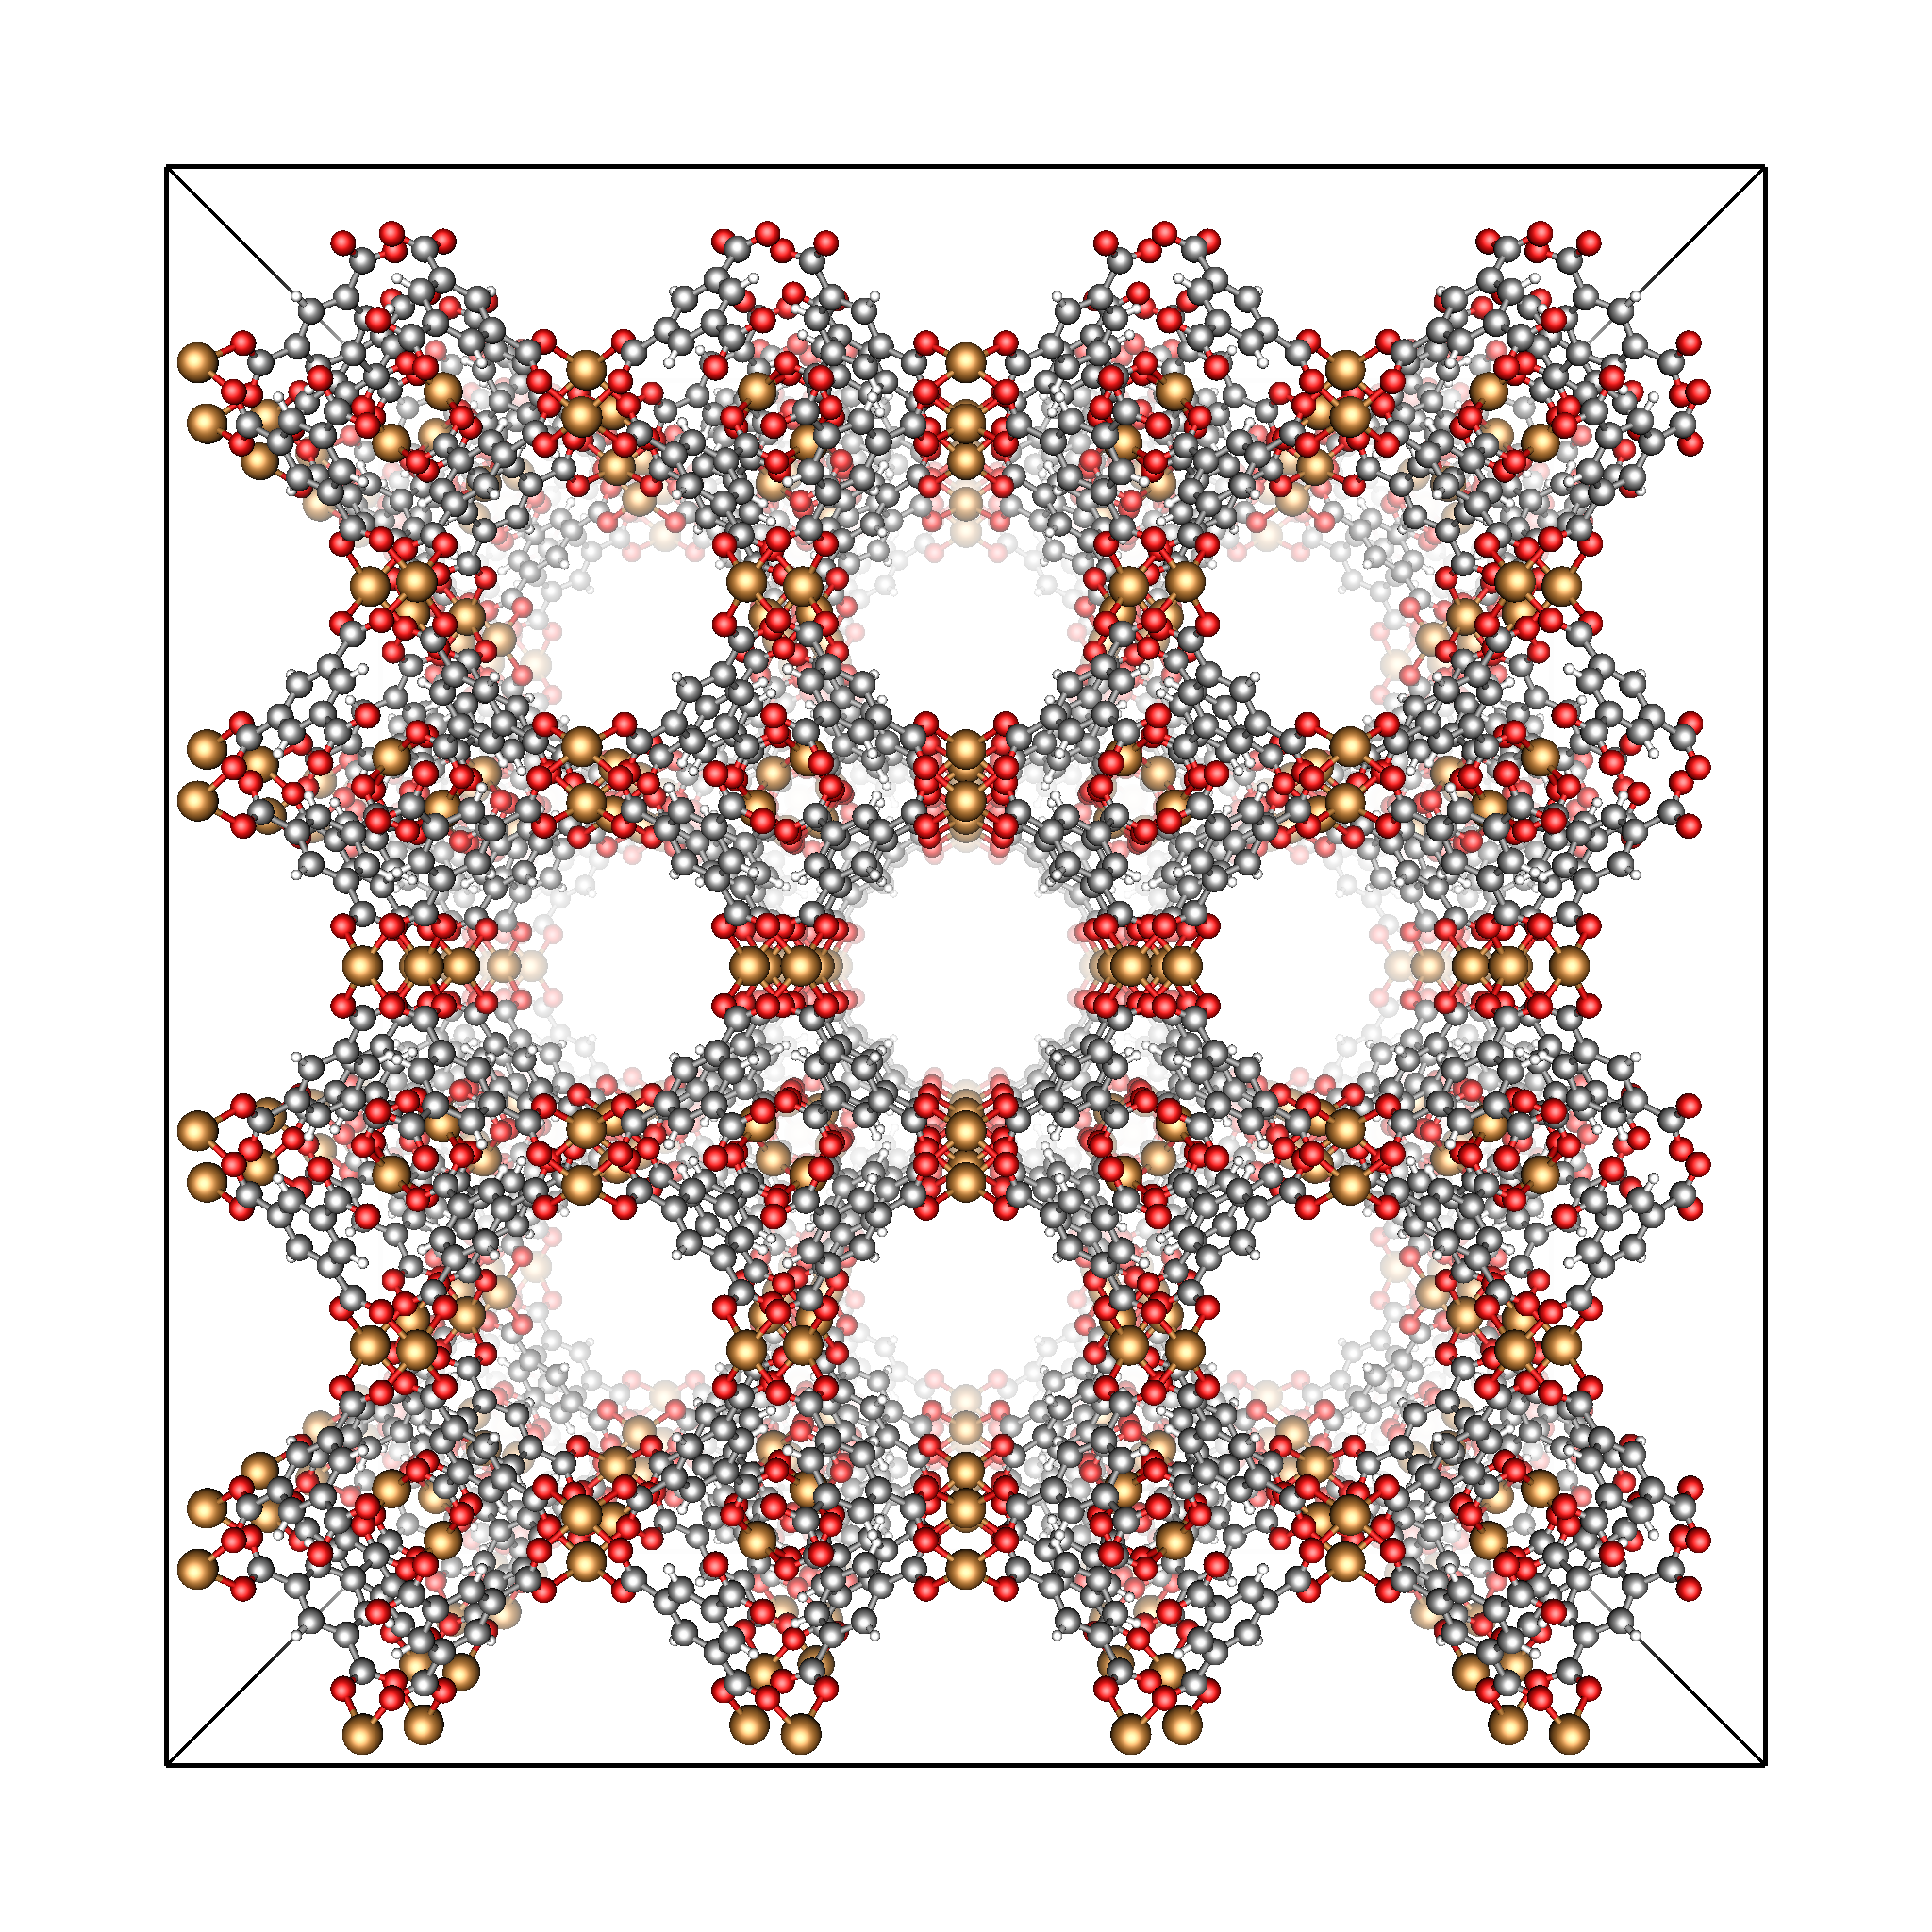
\includegraphics[width=0.6\columnwidth]{hkust-1_fancy.png} \label{fig:example_MOF}
    }
    \qquad
    \subfloat[][]{
        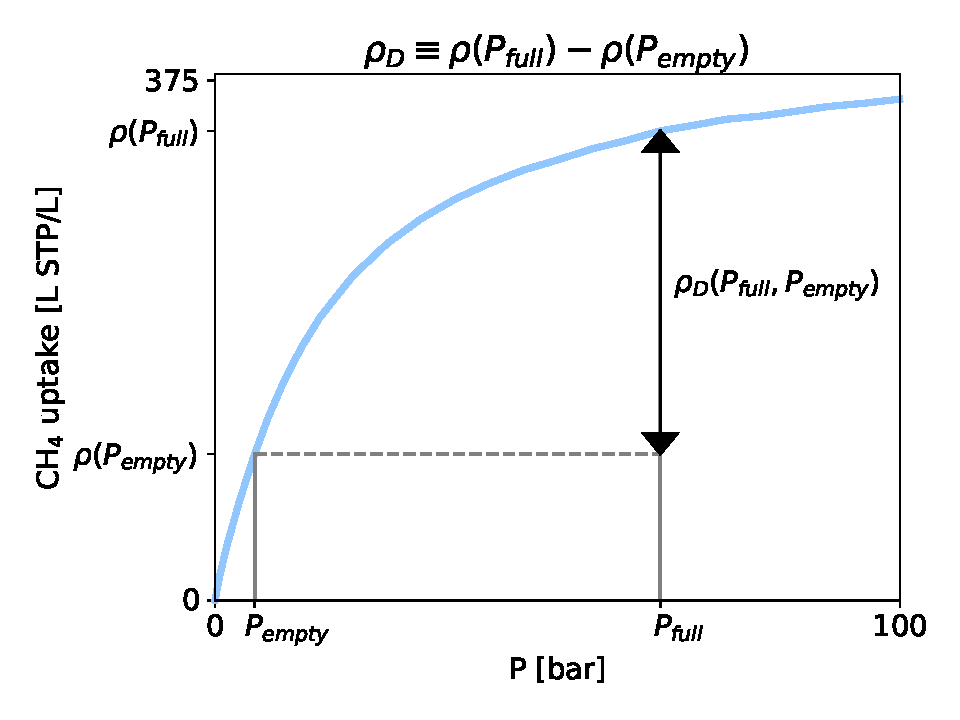
\includegraphics[width=0.98\columnwidth]{usable_capacity_illustration_toy_ish.pdf} \label{fig:delcap}
    }
    \caption{Gas storage and delivery using metal-organic frameworks (MOFs). (a) the crystal structure of an archetype MOF, CuBTC \cite{chui1999chemically}. (b) the methane adsorption isotherm in CuBTC \cite{chui1999chemically} at 298 K (blue) (data from Ref.~\cite{mason2014evaluating}). The deliverable capacity $\rho_D$ is illustrated as the density of gas in the MOF at the storage pressure $\pfull$ minus the density at the discharge pressure $\pempty$.
    }
    \label{fig:fig1}
\end{figure}

To set realistic performance targets and optimally allocate research resources,
in this work, we present a theoretical framework that places an intrinsic upper
limit on the deliverable capacity of any gas in a rigid porous material and
uses as input the experimentally measured properties of the bulk gas. Our
extremum is provided by a substrate that offers a spatially uniform potential
energy field felt by the gas. Applying our framework to methane and hydrogen
gas, we find the US DOE deliverable capacity targets for natural gas and
hydrogen storage and delivery are theoretically possible, but sufficiently
close to the upper bound as to be impractical for any real porous material.
Optimistically, new paradigms outside the scope of applicability of our
theoretical framework, such as gas-induced structural transitions of the
material, hold promise for meeting these targets, as evidenced by flexible MOF
Co(bdp) which currently boasts the largest methane deliverable
capacity~\cite{mason2015methane}.

\section{Gas storage \& delivery by isothermal, pressure-swing adsorption}
Consider a pressure vessel onboard a vehicle (i.e. fuel tank) packed with
porous material. At the filling stage, the tank is connected to a (pure)
gaseous reservoir at pressure $\pfull$ and allowed to equilibrate. At this
point, the adsorbed gas tank is considered full. While driving, gas desorbs
from the adsorbent to the engine/fuel cell, driven by a pressure differential.
The tank is considered depleted/empty when the pressure has dropped to
$\pempty$, the pressure at which the flow rate of gas from the tank to the
engine is insufficient. However, given $\pempty \neq 0$ (pulling vacuum),
residual gas will remain trapped in the adsorbent. Therefore, the driving range
of the vehicle is primarily determined by the \emph{deliverable capacity}. The
isothermal, volumetric deliverable capacity is an intrinsic property of the
nanoporous material and its interaction with the gas.

\section{Review of previous work}
There has been considerable work attempting to establish an upper bound on the
isothermal deliverable capacity in pressure-swing adsorption.

Early work showed that, in the simplified Langmuir model, there exists an
optimal free energy of adsorption (which determines the Langmuir constant) that
maximizes the deliverable capacity
$\rho_D$~\cite{matranga1992storage,bhatia2006optimum,simon2014optimizing}. If
the gas-substrate interaction is too weak (strong), too little (much) gas
adsorbs (is retained) at $\pfull$ ($\pempty$), diminishing $\rho_D$. An upper
bound on the deliverable capacity of a Langmuir material follows if each
adsorption site is endowed with the optimal free energy of adsorption. However,
remaining is the question of how many adsorption sites per volume a porous
material can practically offer, under the constraint that these adsorption
sites provide the optimal free energy of adsorption. Moreover, gas-gas
attractions, neglected in the Langmuir model, could recruit more gas in the
material at $\pfull$ than at $\pempty$ and enhance the deliverable
capacity~\cite{simon2014optimizing}.

G\'omez-Gualdr\'on \emph{et al.}~\cite{gomez2017impact} introduced a model that
accounted for gas-gas interactions via an intermolecular potential and
idealized the substrate in two different ways: (1) discrete adsorption sites
packed into an FCC lattice and (2) a volume endowed with a spatially uniform,
background potential energy field. According to molecular simulation of methane
adsorption, the ARPA-E deliverable capacity target of 315 L STP/L could be
reached in both of these idealized substrates. However, both models neglected
the space occupied by atoms of the porous material that are needed to endow the
adsorption sites/volume with the attractive potential energy.

A third body of work attempted to account for both gas-gas interactions
\emph{and} steric interactions of the gas with the atoms of the porous
material. Simulations of methane adsorption in hundreds of thousands of
explicit nanoporous crystal structures---both real and hypothetical---suggested
that the ARPA-E deliverable capacity target is
infeasible~\cite{simon2015materials}; the highest simulated methane deliverable
capacity was 196 cm$^3$~STP/cm$^3$. Confidence in this conclusion rests upon
(i) the accuracy of the intermolecular potentials describing the molecular
interactions and (ii) the sufficient sampling of material space, i.e.\ that the
structures considered are representative of the set of possible materials. To
further explore material space and address sensitivity to the potentials used,
scaling the Lennard-Jones potential well depths of material atoms to model
enhanced interactions~\cite{gomez2014exploring}, placing Lennard-Jones spheres
in a unit cell randomly to form ``pseudo-materials''~\cite{kaija2018high}, and
generating fictitious potential energy fields via a generative adversarial
network trained on zeolite structures~\cite{lee2019predicting} all generated
model substrates that failed to meet the ARPA-E methane deliverable
capacity target.

% Brown and Freeman \cite{bhown2011analysis}

In this work, we place a rigorous upper bound on the deliverable capacity of a
pure gas in a rigid substrate by endowing a control volume with a spatially
uniform background energy field. Instead of using a molecular model for the
gas~\cite{gomez2017impact}, we use the experimental equation of state to
account for gas-gas interactions. In addition, we prove using the calculus of
variations that this spatially uniform substrate yields a maximal deliverable
capacity. We use our framework to place an upper bound on the deliverable
capacity of methane and hydrogen gas.

\section{An upper bound on the deliverable capacity of a pure gas in a rigid porous material}\label{sec:upper-bound}
\begin{figure}
  \centering
  \includegraphics[width=\columnwidth]{methane-298-rho-mu}
  \caption{The density of bulk methane, the ideal gas, and adsorbed gas in several MOFs at 298\ K as a function of chemical potential (bottom axis) and pressure (top axis). The bulk methane density is from the National Institute of Standards and Technology (NIST)~\cite{nist}. The methane adsorption isotherms in the MOFs are experimental data from Ref.~\cite{mason2014evaluating, furukawa2009storage}.
  }
  \label{fig:density-vs-mu-ch4}
\end{figure}

We now develop a thermodynamic framework that places an upper bound on the deliverable capacity of any pure gas in a rigid porous material.

The thermodynamic properties of a bulk, pure gas are characterized by an
equation of state. Of particular interest for gas storage and delivery is the
density of the gas $\rho_g(\mu,T)$ as a function of chemical potential $\mu$
and temperature $T$, which is shown for methane gas in
Fig.~\ref{fig:density-vs-mu-ch4} at $T=298$\ K. For comparison, we also show
the density of methane adsorbed into several porous materials.

To place an upper bound on the deliverable capacity, consider a substrate whose
sole interaction with the gas is to introduce a spatially uniform potential
energy $\V$ for gas molecules in the control volume (where $\V<0$ for an
attractive potential). Because this interaction is uniform within the
substrate, the gas-gas interactions and thus fluid structure in such a
substrate are identical to those of the pure gas at the same density and
temperature. This allows us to obtain the adsorption properties of this model
substrate using the experimentally measured properties of the pure
gas~\cite{nist}. Intuitively, the deliverable capacity of a gas in such a
homogeneous substrate with the optimal potential energy is an upper bound
because, in a real material, (i) spatial inhomogeneity of the potential
energy results in some points in the control volume offering a suboptimal
attraction for the gas and (ii) the atoms required to create the potential
field exclude gas from occupying a fraction of the control volume.

The spatially uniform potential $\V$ representing gas-substrate interactions
behaves as an external potential and effectively shifts the chemical potential
(or, equivalently, molar Gibbs free energy) of the gas in the material, just as
gravitational potential energy causes the density of air to vary with altitude.
Consequently, the density of gas in our homogeneous substrate is:
\begin{align}
    \rho(\mu,T) &= \rho_g(\mu - \V,T). \label{eq:mof-density}
\end{align}
See Sec.~\ref{sec:V_shifts_chem_pot} for a derivation.

The deliverable capacity of gas in our homogeneous substrate is thus:
\begin{align}
    \rho_D(\V,T) &= \rho(\mufull,T) - \rho(\muempty,T),
    \label{eq:DofPhi}
    \\
    &= \rho_g(\mufull-\V,T) - \rho_g(\muempty-\V,T),
\end{align}
where $\mufull$ and $\muempty$ are the chemical potentials corresponding to the
pressures $\pfull$ and $\pempty$, respectively. Thus, $\rho_D$ for our
homogeneous substrate as a function of $\V$ is the difference between two
shifted versions of $\rho_g(\mu; T)$. Figure~\ref{fig:methane-298-D} shows the
two shifted bulk methane density curves and their difference. The horizontal
axis is the difference in molar Gibbs free energy at fixed density and
temperature between the gas within the substrate and the pure gas (\gst), which
is equal to $\V$ in our model. We see a potential $\V$ that maximizes the
deliverable capacity of our ideal substrate, balancing the need to maximize the
density at $\pfull$ against the need to minimize residual gas retained at
$\pempty$.

The optimal deliverable capacity of methane (298\ K, $\pfull=$ 65\ bar,
$\pempty=$ 5.8\ bar) in our ideal, spatially uniform substrate is 374\ L STP/L,
achieved for $\V_{opt} =$ 5.9\ kJ/mol.

An essential question is whether our idealized substrate, with spatially
uniform potential $\V_{opt}$ for the gas, places an upper bound on the
deliverable capacity in all rigid porous materials. In the SI (see
Section~\ref{sec:proof-extremum}), we show that our idealized substrate with
spatially uniform potential $\V_{opt}$ yields an \emph{extremum} of the
deliverable capacity over all possible \emph{static potential energy fields},
provided the gas does not crystallize at the temperature and in the density
range of interest. The potential energy field is \emph{static} if it is
unaffected by the presence of the gas; consequently, our model does not apply
to flexible materials that undergo gas-induced conformation
changes~\cite{schneemann2014flexible}. We next argue that this extremum is a
maximum by addressing two alternative possibilities: the extremum could turn
out to be (i) a saddle point or (ii) a local, rather than global, maximum.

Fig.~\ref{fig:methane-298-D} clearly shows that $\V_{opt}$ provides a maximum $\rho_D$ over all \emph{spatially uniform}, static potential energy fields. To qualitatively argue that the spatially uniform potential $\V_{opt}$ provides a maximum deliverable capacity over \emph{all} (including non-spatially uniform) static potential energy fields (a broader claim), consider a non-spatially-uniform variation on $\V_{opt}$.
We will show that the effect of this variation is to reduce the deliverable capacity.
At low adsorbed gas densities, the lowest-energy positions will be preferentially occupied, while at higher densities, the additional gas molecules will be forced into higher energy locations. Thus, the mean attraction will be lowest at \pfull\  and highest at \pempty.  This will result in $\gst$ increasing monotonically with with pressure.  As shown in the Supplementary Information (see Sec.~\ref{sec:monotonic}), this results in the deliverable capacity of a non-uniform potential being lower than the deliverable capacity of a uniform potential with $\V=\gst$ for either $\pfull$ or $\pempty$.
Thus a spatially uniform potential will give the best deliverable capacity amongst all static potential energy fields that give the same $\gst$, and the \emph{optimal} uniform potential $\V_{opt}$ will give the a greater deliverable than any static non-uniform potential.

\begin{figure}
    \centering
    \includegraphics[width=0.95\columnwidth]{methane-298-n-vs-G}
    \caption{The deliverable capacity of methane as a function of the attractive Gibbs free energy $|\gst|$.
    Experimental deliverable capacities for several MOFs (data from Ref.~\cite{mason2014evaluating, furukawa2009storage}) are shown along with the experimental values for $\gst$ at the empty and full pressures shown as dots connected by a line (not visible at this scale).}
    \label{fig:methane-298-D}
\end{figure}

\section{Results}
Although our theoretical framework allows us to place an upper bound on the deliverable capacity of many different gases in a rigid porous material, we focus on the maximal deliverable capacity of methane and hydrogen gas in our homogeneous substrate due to their application as transportation fuels. To characterize the density of the gases, $\rho_g(p, T)$, we use experimental data from NIST~\cite{nist}, which naturally includes quantum effects that particularly affect hydrogen at low temperature~\cite{kumar2006quantum}. In the context of storage onboard passenger vehicles, we compare our upper bound with several prominent porous materials using experimental adsorption isotherms from the literature; we also compare with deliverable capacity targets set by the US DOE.

Figure~\ref{fig:methane-298-D} shows the upper bound for methane storage at room temperature~(374~cm$^3$~STP/cm$^3$). In addition to the predicted maximum deliverable capacity as a function of \gst,
\corysays{subtlety here: isnt ur proof restricted to saying $\V_{opt}$ provides the upper bound? does it really prove that, for fixed and nonoptimal $\gst$, a spatially uniform potential is optimal over a non-spatially uniform one? I don't think it does...}
the ARPA-E target of 315~cm$^3$~STP/cm$^3$~\cite{arpaemove} is shown for context. For an adsorbent with at least 84\% void fraction, the ARPA-E target is theoretically possible. The experimental deliverable capacities of several adsorbents~\cite{mason2014evaluating} are also shown over a range of $\gst$ (converted from the measured adsorption isotherm as explained in Sec.~\ref{sec:phi-is-delta-g}). These can be compared with the highest observed deliverable capacities for methane at room temperature in rigid materials, up to 208~cm$^3$~STP/cm$^3$~\cite{simon2015materials}. 
% don't think the below is helpful or correct: Gst opt is reached by some... there are void fraction constraints too.
% To reach the ARPA-E target, an adsorbent material with a higher $|\gst|$ would need to be found. 

\begin{figure}
    \centering
    \includegraphics[width=0.95\columnwidth]{hydrogen-298-n-vs-G}
    \caption{Deliverable capacity of hydrogen at room temperature as a function of the attractive Gibbs free energy $|\gst|$.  Experimental deliverable capacities for several MOFs are shown along with the experimental values for $\gst$ at the empty and full pressures shown as x's connected by a line.}
    \label{fig:hydrogen-298-D}
\end{figure}

\corysays{Figs.~\ref{fig:hydrogen-298-D} ~\ref{fig:methane-298-D} why not just let $\gst$ be negative and have an arrow pointing in direction of more attraction? as written the legend is not correct since those are not the functions being shown. in the main text we never discussed what \gst is for the MOF and why the MOFs are lines not points (\gst is a function of density now)
\jpsays{due to a different deliverable capacity at full pressure and empty pressure. For hydrogen the SI (by Paula Garcia-Holley) has total uptake plots so we could make a curve even but would have a lot of error due to manual extraction?}}

Storage of hydrogen is considerably more challenging owing to its relatively weak interaction with adsorbents. The DOE ULTIMATE deliverable capacity target~\cite{DOE} is within 6\% of the upper bound at 25$^\circ$C. Figure~\ref{fig:hydrogen-298-D} shows the theoretical upper bound curve for hydrogen storage along with a range of experimental measurements for known MOFs.  The DOE ULTIMATE deliverable capacity target is theoretically possible, however by such a small margin that we can safely rule out the possibility of reaching this target through storage and delivery of hydrogen in \emph{any} rigid substrate at room temperature. Such a material would require a void fraction of at least 94\%. On top of this, the DOE ULTIMATE target requires an optimal $|\gst|$ of 10~kJ/mol which is far greater than what is found in observed porous materials. This reflects the known fact that hydrogen interacts with substrates far more weakly than methane does. One possibility that has been pursued is storage at cryogenic temperatures. See Section~\ref{sec:cryo-hydrogen} in the Supplementary Information for the upper bound for storage of hydrogen at 77 K.

Why do we not experimentally observe materials approaching the upper bound on the deliverable capacity? Foremost, any adsorbent substrate will be composed of atoms, which will exclude the gas from some volume. Due to strong short-range interactions, substrate atoms must be uniformly distributed to achieve strong attraction for gas atoms. Uniform atom distribution sets a limit on the pore volume.
% Because strong interactions are short-range, achieving a strong attraction requires that substrate atoms be distributed throughout the volume, which places a limit on the pore volume.
In contrast, real materials have a spatially non-uniform attraction for gas atoms. The result of this is that there are regions of space with non-optimal attraction. For hydrogen, there is the further issue that there are \emph{no} known physical interactions that are sufficiently strong to give an optimal deliverable capacity at room temperature.
% Finally, real materials must have a spatially non-uniform attraction for gas atoms, resulting in some regions of space where the attraction is not optimal. For hydrogen, there is the further issue that there are \emph{no} known physical interactions that are sufficiently strong to give an optimal deliverable capacity at room temperature.

\section{Conclusion}
We have established an upper bound on the deliverable capacity via pressure-swing adsorption in rigid porous solids based on experimentally measured properties of pure gases. While these upper bounds do not rule out the discovery of materials that reach current DOE targets, they cast strong doubt on the possibility of achieving these goals when we consider the additional constraints imposed due to steric hindrance between substrate atoms and the adsorbate. Our upper bound does indicate that those goals cannot be exceeded by more than 16\% for methane and 6\% for hydrogen. Fortunately, there are some limitations to these upper bounds which suggest avenues for future developments which could allow the targets to be met.

The first limitation of our proof is that we restricted ourselves to \emph{isothermal} pressure swing storage. By raising the temperature of the adsorbent during gas discharge to drive off residual gas~\cite{gomez2014exploring}, the deliverable capacity could be enhanced, albeit at the cost of a more complicated engineering design of the fuel tank and vehicle.

The second limitation of our proof arises in the assumption of a rigid substrate. The rigid substrate acts as a static potential energy field for gas molecules that is unchanged by the adsorption of gas.
% The second limitation of our proof arises in the assumption of a rigid substrate, which acts as a static potential energy field for gas molecules that is unchanged by the adsorption of gas.
For most porous materials this is a reasonable approximation, and this assumption is frequently made in both the simulation and theory of porous materials~\cite{witman2017influence}. However, there are cases where the substrate can in effect provide a very strongly gas-density-dependent interaction through structural flexibility~\cite{schneemann2014flexible}. A flagship example is MOF Co(bdp)~\cite{choi2008broadly}, which possesses a wine-rack-like topology capable of hinge motion. At low methane pressure, Co(bdp) adopts a collapsed, nonporous state, but expands to a porous state and fills with gas at higher pressures~\cite{mason2015methane}. This allows Co(bdp) to fully expel its residual gas at low pressures.
Our upper bound does not consider such material effects and thus flexible materials could have significantly higher deliverable capacities.
% Such materials can indeed violate our upper bound and thus could lead to significantly improved deliverable capacities.

We note that our upper bound can readily be applied to the storage of other gasses of interest, with the proviso that the gas is far from crystallization. Our code is available at \davidsays{XXXXX}.


% general conclusion linking all manuscripts
\chapter{General Conclusion}

In the first manuscript \emph{Stochastic approximation Monte Carlo with a dynamic update factor}, we developed and refined the novel Monte Carlo method SAD. We compared the convergence properties of SAD to a variety of other weight-based flat-histogram methods. We also examined the convergence behavior applied to the square-well fluid and a Lennard-Jones cluster.

In the second manuscript \emph{Flat-histogram method comparison on 2D Ising model}, we tested SAD on the 2D Ising model against a number of weight-based methods including a ``production'' run WL. We found that even for systems where it is convenient to choose an energy range, SAD performs incredibly well.

In the third manuscript \emph{An upper bound to gas delivery via pressure-swing adsorption in nanoporous materials}, we develop an upper bound on gas delivery and compare the theory with experimental data. We found that while hydrogen may not be viable at room temperature, methane storage can potentially meet the Department of Energy (DOE) targets. The theory also suggests an ideal energy of attraction which will help when determining what MOFs to simulate.

Each of these manuscripts laid the groundwork for the development of 2D SAD. SAD has been tested on a variety of physical systems and shows tremendous promise for simulating isotherms. In addition, an upper bound was developed that will aid in simulating MOFs using 2D Sad.

There are two important steps that remain to complete the extension.  The first is the development of SAD with a minimum particle number $N_{\min}$ instead of a $T_{\min}$. By varying the number of particles, the simulation can yield thermodynamic insights for all densities. The second step that remains is the merger of each SAD method such that a multidimensional 2D SAD is formed. Such a Monte Carlo method would be an invaluable tool for driving research in the gas storage field.

\printbibliography[title={Bibliography}]

\clearpage{}

\appendix
\chapter{Appendix}
\setcounter{table}{0}
\renewcommand{\thetable}{S\arabic{table}}%
\setcounter{figure}{0}
\renewcommand{\thefigure}{S\arabic{figure}}%
\renewcommand{\thesection}{SI~\Alph{section}}%

\section{An external, spatially uniform potential $\V$ shifts the chemical potential $\mu$ of the gas} \label{sec:V_shifts_chem_pot}
We show that imposing an external, spatially uniform potential $\V$ to a gas
has the effect of shifting the chemical potential $\mu$ of the gas, recovering
eqn.~\ref{eq:mof-density}. Consider a control volume $\Omega$ with volume
$V=|\Omega|$ (large enough to neglect boundary effects) that is endowed with
the external, spatially uniform potential $\V$. Impose the grand-canonical
ensemble, where this control volume can exchange energy and particles with a
bath of gas at temperature $T$ and chemical potential $\mu$.

To denote a microstate of this system, let $N$ be the number of gas particles
in the control volume and $\mathbf{r}_1,...,\mathbf{r}_N$ be their positions.
Then, the potential energy $E$ of a microstate of the control volume is:
\begin{equation} E(\rvec_1,...,\rvec_N) = N\V +
E_{gg}(\rvec_1,...,\rvec_N), \end{equation} where $E_{gg}$ is the
(unknown and complicated) interatomic potential for gas-gas
interactions that governs the (real) gas properties. The first term
arises from each gas molecule experiencing the external potential
$\V$, where $\V < 0$ corresponds to attraction.  To account
  for molecular rotational and vibrational degrees of freedom, we
  could treat the positions $\rvec_i$ as the locations of atoms rather
  than molecules.  In this case the gas-gas interactions will include
  both \emph{intra-molecular} interactions and \emph{inter-molecular}
  interactions.

The grand canonical partition function of the control volume is:
\begin{multline}
    \Xi(\mu, V, T)= \\ \displaystyle \sum_{N=0}^\infty \frac{1}{\Lambda^{3N}N!} \int_{\Omega} \cdots \int_{\Omega} e^{-\beta E_{gg}(\rvec_1, ..., \rvec_N)} e^{\beta (\mu - \V) N} d\rvec_1 \cdots d\rvec_N.
    \label{eq:gcpf}
\end{multline}
We recognize this as the grand canonical partition function of the bulk gas in
the control volume without the external potential, but shifted in chemical
potential:
\begin{equation}
    \Xi(\mu, V, T)=\Xi_0(\mu - \V, V, T)
    \label{eq:xi_vs_xi0}
\end{equation}
where $\Xi_0(\mu, V, T)$ is the grand partition function of the bulk
gas in the control volume in the absence of an external potential. Importantly,
this equivalency depends on the potential $\V$ being spatially uniform.
Therefore, the thermodynamic properties of the gas atoms in the spatially
uniform external potential $\V$ (adsorbed in our idealized substrate)
are equivalent to the properties of the bulk gas at chemical potential $\mu-\V$
(where $T$ is held fixed). As $\V$ becomes more negative, corresponding to a
more attractive adsorbent, the thermodynamic properties of the adsorbed gas in
our ideal substrate are equivalent to the gas at a higher chemical potential.

\section{Proof of extremum}\label{sec:proof-extremum}
To show that a uniform potential gives the highest deliverable capacity, we
consider an interaction potential between gas and substrate $\V(\rvec)$ that
varies in space.  In this proof, we make use of the Fourier transform of
this potential:
\begin{align}
    \Vk \equiv \iiint \V(\rvec) e^{-i\kvec\cdot \rvec} d\rvec
\end{align}
The Fourier transform of a uniform potential is a Dirac delta function $\tilde{\V}(\kvec)\propto\delta(\kvec)$. In order for a uniform potential
to extremize the deliverable capacity, we must show that the functional
derivative of the deliverable capacity with respect to $\Vk$ is zero for
\emph{nonzero} values of $\kvec$, i.e.
\begin{align}
    \frac{\delta D}{\delta \Vk} &= 0, \text{ if } \kvec\ne 0.
\end{align}
We note that this functional derivative may be non-zero for $\kvec=0$ because
we separately maximize with respect to the particular uniform potential $\V$.
This means that
\begin{align}
    \frac{\delta N_H}{\delta \Vk} &= \frac{\delta N_L}{\delta \Vk}
\end{align}
where $N_H$ and $N_L$ are the number of particles at the low and high pressure.

Because the chemical potential $\mu$ varies monotonically with $N$ at fixed
temperature, we can consider how the chemical potential varies as we change
$\Vk$ with the number of molecules held fixed. We demonstrate this using the
cyclic chain rule, which shows us that
\begin{align}
    \left(\frac{\delta N}{\delta \Vk}\right)_{\mu} &=
    -\left(\frac{\delta \mu}{\delta \Vk}\right)_{N}
    \left(\frac{\partial N}{\partial \mu}\right)_{\Vk}.
\end{align}
Since changing the chemical potential changes the number of molecules in the general case, if we can show that $\left(\frac{\delta \mu}{\delta \Vk}\right)_{N}=0$ then we will have shown that $\left(\frac{\delta N}{\delta \Vk}\right)_{\mu}=0$.  Thus we consider
\begin{align}
    \left(\frac{\delta \mu}{\delta \Vk}\right)_N
    &= \left(\frac{\delta \left(\frac{\partial F}{\partial N}\right)_{\volume}}{\delta \Vk}\right)_N
    \\
    &= \left(\frac{\partial \left(\frac{\delta F}{\delta \Vk}\right)_{\volume}}{\partial N}\right)_{\volume}
    \label{eq:dmudpot}
\end{align}
where we have made use of the derivative relationship between $\mu$ and the Helmholtz free energy $F$, and have then reordered the functional and partial derivatives.
Let us consider the interior derivative first.  The derivative of the Helmholtz free energy with respect to the external potential $\Vk$ yields the number density:
\begin{align}
    \frac{\delta F}{\delta \Vk} &= \rho(\kvec)
\end{align}
The number density is itself spatially uniform for any stable system in a fluid state at this density (i.e. does not spontaneously crystallize), and thus has a Fourier transform that is proportional to a Dirac $\delta$-function.  Thus, the functional derivative $\frac{\delta F}{\delta \V(\rvec)}$ is actually a uniform function.
We can insert this expression into Eq.~\ref{eq:dmudpot} to find that
\begin{align}
    \left(\frac{\delta \mu}{\delta \Vk}\right)_N &\propto \delta(\kvec) \\
    \left(\frac{\delta N}{\delta \Vk}\right)_\mu &\propto \delta(\kvec)
\end{align}
Thus, the functional derivative of both $\mu$ and $N$ with regard to $\V(\rvec)$ are themselves spatially uniform.  Since we already maximize $D$ with respect to the spatially uniform component of the potential (i.e. $\kvec=0$), the derivative of $D$ with respect to any change of potential is zero.

This demonstrates that a spatially uniform potential leads to an extremum value
of the deliverable capacity. This proof is insufficient, however, to show that
it must be a true maximum.

\section{The real-substrate analog of $\V$ is $\gst$}
\label{sec:phi-is-delta-g}
\begin{figure}
    \centering
    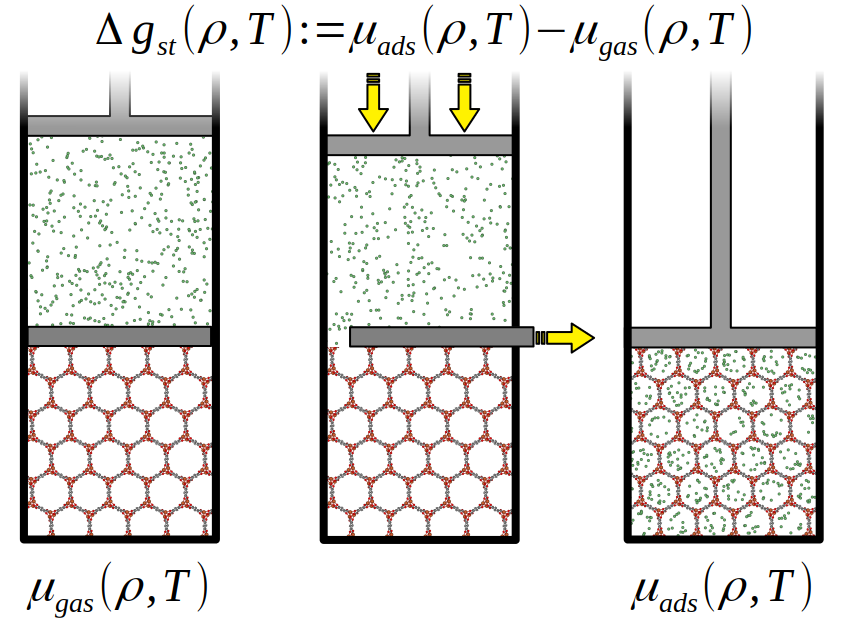
\includegraphics[width=\columnwidth]{g_st_piston_2.png}
    \caption{Cartoon illustrating the definition of $\gst$ and a
      hypothetical experiment to measure it with a piston and
      removable barrier that separates two equal volumes, one with a
      porous material (bottom) and one with free space (top). The
      initial state (left) is a bulk gas phase at density $\rho$ and
      temperature $T$. An infinitely-thin, removable barrier separates
      the gas from the porous material (bottom). The barrier is then
      slowly removed, and the piston slowly pushes all gas molecules
      into the porous material in an isothermal process. The final
      state (right) is an adsorbed gas phase at density $\rho$ and
      temperature $T$.}
    \label{fig:delta-G-cartoon}
\end{figure}

The parameter describing our idealized substrate is $\V$, the spatially uniform
potential felt by a gas molecule adsorbed in the idealized substrate. A natural
question is how this potential relates to the properties of real substrates.
The effect of $\V$ in our model is to shift the chemical potential $\mu$ of the
gas (see Sec.~\ref{sec:V_shifts_chem_pot}). Because our ideal substrate shifts
the chemical potential of the gas molecules by providing a spatially uniform
potential energy field, the entropy of the gas in the ideal substrate is equal
to the entropy of the gas in its bulk state at the same density and
temperature. In contrast, a real substrate provides a non-spatially uniform
potential. Consequently, the entropy of the gas inside a real substrate is
\emph{not} equal to the entropy of the bulk gas at the same density and
temperature. Therefore, the parameter analogous to $\V$ in a real substrate
will involve both energy and entropy. The real-substrate analog of $\V$ is the
shift of molar Gibbs free energy provided by the substrate, specifically an
\emph{isosteric} (or constant-density) shift of the Gibbs free energy:
\begin{equation}
   \gst(\rho, T) \equiv
   %\frac{G_{\text{ads}}(\rho, T) - G_{\text{gas}}(\rho, T)}{N}\\ 
    \mu_{\text{ads}}(\rho, T) - \mu_{\text{gas}}(\rho, T).
  % \gst(\rho, T) &\equiv g_{\text{gas}}(\rho, T) - g_{\text{ads}}(\rho, T)
  \label{eq:g_st}
\end{equation}
The isosteric Gibbs free energy difference $\gst$ is the difference in molar
Gibbs free energy (equivalent to chemical potential) between the adsorbed gas system and
the bulk gas \emph{with the same density of gas molecules}. The quantity $\gst$
does \emph{not} correspond to a change in the molar Gibbs free energy as a
molecule is adsorbed, which is zero under conditions of coexistence. The
quantity $\gst$ in a real substrate is a direct analog to $\V$ in our ideal
substrate because it is the chemical potential shift needed to impose on the
bulk gas in coexistence with the real substrate to achieve the same density as
in the substrate (compare with eqn.~\ref{eq:xi_vs_xi0}).
Figure~\ref{fig:delta-G-cartoon} illustrates a hypothetical experiment to
measure $\gst$ via a piston with a removable partition that separates a volume
of free space from the same volume of substrate. Note that $\gst$ is a property
of both the substrate and the identity of the gas. Because real substrates
offer a \emph{non}-spatially uniform potential, $\gst(\rho, T)$ is a function
of $\rho$ and $T$, unlike our ideal, homogenous substrate where $\gst(\rho,
T)=\V$. Consequently, throughout this article, we show $\gst(\rho, T)$ for real
substrates at both conditions relevant to gas storage and delivery, $\pfull$
and $\pempty$.

In practice, we can readily compute $\gst(\rho, T)$ of a real gas/substrate
system from (i) the (experimental or simulated) equilibrium adsorption isotherm
of the gas in the substrate and (ii) the (experimental or simulated) chemical
potential of the bulk gas. Consider the real substrate in thermodynamic
equilibrium with a bulk gas at fixed temperature $T$ and pressure $p$, and let
$\rho=\rho(p, T)$ be the density of gas in the substrate. At coexistence, the
chemical potential of the bulk gas is equal to the chemical potential of the
adsorbed gas in the substrate. Thus, we can use the experimentally known molar
Gibbs free energy of the pure, bulk gas system at temperature $T$ and pressure
$p$ to determine the molar Gibbs free energy of the adsorbed system:
$\mu_{\text{ads}}(\rho, T)=\mu_{\text{gas}}(p, T)$. We can then also look up
the known chemical potential of the bulk gas at the same density and
temperature as in the substrate, $\mu_{\text{gas}}(\rho, T)$. Via
eqn.~\ref{eq:g_st}, $\gst$ follows from subtracting the two quantities.

An interesting question is how $\gst$ relates to the commonly measured and
reported isosteric heat of adsorption $q_{st}$, which is roughly the energy
change when a gas molecule is adsorbed~\cite{sircar1999isosteric,
tian2017differential}. Figure~\ref{fig:qst-vs-delta-G} shows how $q_{st}$
compares to $\gst$ for several prominent adsorbents. In every case,
$|q_{st}|>|\gst|$ because the gas in the adsorbent always has less entropy than
the gas in the bulk at the same density and temperature. That is, while
adsorption is energetically favored, it is entropically disfavored due to the
restrictions imposed on the configuration of the gas molecules via steric
interactions with the substrate itself; this counters the energetic attraction.

\begin{figure}
    \centering
    \includegraphics[width=0.95\columnwidth]{qst-vs-delta-G}
    \caption{Relationship between $\gst$ and the isosteric heat
      $q_{st}$ for several prominent adsorbents at room
      temperature (data from Ref.~\cite{mason2014evaluating, garcia2018benchmark}). The dots represent the properties of methane
      adsorption at 5.8~bar and 65~bar. The $+$'s represent the
      properties of hydrogen adsorption at 5~bar and
      100~bar.}
    \label{fig:qst-vs-delta-G}
\end{figure}

\begin{figure}
    \centering
    \includegraphics[width=0.95\columnwidth]{methane-298-gst}
    \caption{The density-dependence of $\gst$ of methane in several
      adsorbents (298\ K). Note that $\gst$ is monotonic in
      $\rho$. Data from
      Refs.~\cite{mason2014evaluating, furukawa2009storage}.
    }
    \label{fig:methane-gst}
\end{figure}

\begin{figure}
    \centering
    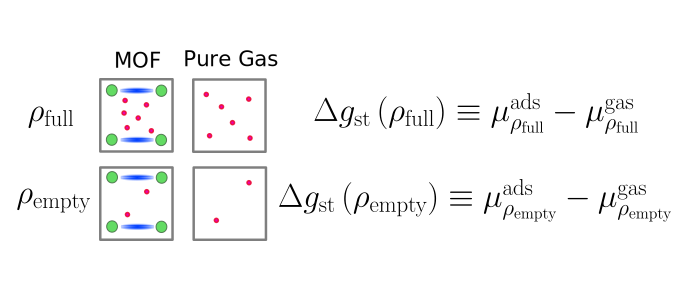
\includegraphics[width=0.95\columnwidth]{four-cases-pro}
    \caption{Two pairs of boxes containing gas with one of the pairs
    filled with MOF. One box of each sort has a density of gas $\rhofull$
    corresponding to $\pfull$ in the MOF system, while the other two boxes has
    gas density $\rhoempty$}
    \label{fig:delta-gst-maximum}
\end{figure}

\section{An upper bound when $\gst(\rho)$ is monotonic}\label{sec:monotonic}
Every MOF has a $\Delta g_\text{st}$ at $\pfull$ and $\pempty$ corresponding
to a full and empty density. The deliverable capacity of the MOF is equal to
the difference between the full and empty density. Examining
Fig.~\ref{fig:methane-gst}, we see that a significant variety of known
experimental $\Delta g_\text{st}$ curves are monotonic. Furthermore, our
qualitative argument in Section~\ref{sec:upper-bound} suggests that this
function \emph{should} monotonically increase for rigid substrates, as
increasing the density of gas causes some of the gas to reside in higher-energy
sites. If this is always the case, the deliverable capacity will always be
bounded by our theoretical upper bound, even for a value of $\V$ that is not
optimal.

To show this, we perform a thought experiment illustrated in
Fig.~\ref{fig:delta-gst-maximum}. We begin with two pairs of boxes containing
gas. Two of the boxes are filled with a MOF, and the other two have a uniform
potential energy $\V$. We imagine the two boxes at $\V$ as being empty
but at very low altitude where gravity provides a potential energy difference
(relative to the box with the MOF in it) of $\V$ to each gas molecule (perhaps
we are on Jupiter?). One box of each sort has a density of gas $\rhofull$
corresponding to $\pfull$ in the MOF system, while the other two boxes has gas
density $\rhoempty$.

We now consider what happens if we introduce a diffusive connection between two
boxes that are initially at the same density, for instance by connecting them
with a tube. If the chemical potential of the two boxes are equal, their
density will be unchanged, otherwise gas will flow into the box with lower
chemical potential. The difference in chemical potential is equal to the
difference
\begin{align}
   \gst(\rho) - \V &= \left(\mu_{\text{MOF}}(\rho) - \mu_{\text{gas}}(\rho)\right)
   - \left(\mu_{\V}(\rho) - \mu_{\text{gas}}(\rho)\right)
   \\
   &= \mu_{\text{MOF}}(\rho) - \mu_{\V}(\rho).
\end{align}
Thus if $\gst(\rhoempty) = \V$ then the ``empty'' containers will remain at
their initial density after they are connected. Thus, the deliverable capacity
of the MOF will be greater than the deliverable capacity of the model with
uniform potential $\V$ if and only if $\gst(\rhofull)<\V$, i.e. if $\gst(\rho)$
does \emph{not} monotonically increase. By the same token, if we consider the
case where $\gst(\rhofull) = \V$, then to achieve a greater deliverable
capacity than our model, the MOF must have less residual gas, which means that
gas must spontaneously flow from the low-density MOF to the box with potential
$\V$, which means that $\gst(\rhoempty)>\V$. Once again, exceeding our upper
bound requires a material with a $\gst(\rho)$ that does not increase
monotonically.

Taken together, this indicates that not only is our absolute upper bound an
upper bound for rigid MOFs, but the green curve labeled $\rho_D(\gst)$ in
Figs.~\ref{fig:methane-298-D}, \ref{fig:hydrogen-298-D}, and
\ref{fig:hydrogen-77-D} is an upper bound for materials with a non-optimal
$\gst$ at either $\pfull$ or $\pempty$.

\section{Cryogenic hydrogen storage}\label{sec:cryo-hydrogen}
\begin{figure}
    \centering
    \includegraphics[width=0.95\columnwidth]{hydrogen-77-n-vs-G}
    \caption{Deliverable capacity of hydrogen at 77\ K as a function of the attractive Gibbs free energy $\gst$. Experimental deliverable capacities for several MOFs (data from Ref.~\cite{garcia2018benchmark}) are shown along with the experimental values for $\gst$ at the empty and full pressures shown as $+$'s connected by a line.}
    \label{fig:hydrogen-77-D}
\end{figure}

One approach to increase the deliverable capacity is to reduce the storage
temperature. This is illustrated in Fig.~\ref{fig:hydrogen-77-D}, which shows
the upper bound to the deliverable capacity of hydrogen at 77\ K, the boiling
point of nitrogen. The DOE ULTIMATE target in this case looks far more
achievable, and with a much lower $|\gst|$. In fact, an empty tank at this
temperature can satisfy the DOE 2020 target. The DOE ULTIMATE target is 14\%
below the upper bound. Actual MOFs fall far short of the theoretical maximum.

%\printindex
\end{document}
